%%%%%%%% ICML 2026 EXAMPLE LATEX SUBMISSION FILE %%%%%%%%%%%%%%%%%

\documentclass{article}

% Recommended, but optional, packages for figures and better typesetting:
\usepackage{microtype}
\usepackage{graphicx}
\usepackage{subcaption}
\usepackage{booktabs} % for professional tables

% hyperref makes hyperlinks in the resulting PDF.
% If your build breaks (sometimes temporarily if a hyperlink spans a page)
% please comment out the following usepackage line and replace
% \usepackage{icml2026} with \usepackage[nohyperref]{icml2026} above.
\usepackage{hyperref}
\usepackage{enumitem}

% Attempt to make hyperref and algorithmic work together better:
\newcommand{\theHalgorithm}{\arabic{algorithm}}

% Use the following line for the initial blind version submitted for review:
\usepackage[preprint]{icml2026}

% For preprint, use
% \usepackage[preprint]{icml2026}

% If accepted, instead use the following line for the camera-ready submission:
% \usepackage[accepted]{icml2026}

\usepackage{amsmath}
\usepackage{amssymb}

\usepackage{amsthm}
\usepackage{amsfonts}
\usepackage{mathrsfs}
\usepackage{bbm}

\usepackage{mathtools}
\mathtoolsset{showonlyrefs=true}

%%%%%%%%%%%%%%%%%%%%%%%%%%%%%%%%
% THEOREMS
%%%%%%%%%%%%%%%%%%%%%%%%%%%%%%%%
\theoremstyle{plain}
\newtheorem{theorem}{Theorem}[section]
\newtheorem{proposition}[theorem]{Proposition}
\newtheorem{lemma}[theorem]{Lemma}
\newtheorem{corollary}[theorem]{Corollary}
\theoremstyle{definition}
\newtheorem{definition}[theorem]{Definition}
\newtheorem{assumption}[theorem]{Assumption}
\theoremstyle{remark}
\newtheorem{remark}[theorem]{Remark}
\newtheorem{example}[theorem]{Example}

% Todonotes is useful during development; simply uncomment the next line
%    and comment out the line below the next line to turn off comments
%\usepackage[disable,textsize=tiny]{todonotes}
\usepackage[textsize=tiny]{todonotes}

% Define math operators
\DeclareMathOperator*{\argmax}{argmax}
\DeclareMathOperator*{\argmin}{argmin}
\DeclareMathOperator{\tr}{tr}
\DeclareMathOperator{\vect}{vec}
\DeclareMathOperator{\Rank}{Rank}

% Define shortcut
% Define math operators
% \DeclareMathOperator*{\argmax}{argmax}
% \DeclareMathOperator*{\argmin}{argmin}
% \DeclareMathOperator{\tr}{tr}
% \DeclareMathOperator{\vect}{vec}
% \DeclareMathOperator{\Rank}{Rank}

% Define shortcut
\newcommand{\E}{\mathbb{E}}
\newcommand{\B}{B}
\newcommand{\Var}{\mathrm{Var}}
\newcommand{\Cov}{\mathrm{Cov}}
\newcommand{\bbm}[1]{\mathbbm{#1}}
\newcommand{\bb}[1]{\mathbb{#1}}
\newcommand{\floor}[1]{\lfloor #1 \rfloor}
\newcommand{\sq}[1]{\textquoteleft #1 \textquoteright}
\newcommand{\dq}[1]{\textquotedblleft #1 \textquotedblright}
\newcommand{\red}{\color{red}}
\newcommand{\norm}[1]{\left\lVert#1\right\rVert}
\def\T{{\textsc{t}}}

\newcommand{\pr}{\textup{pr}}
\newcommand{\cov}{\textup{cov}}
\newcommand{\var}{\textup{var}}
\newcommand{\avar}{\textup{avar}}
\newcommand{\acov}{\textup{acov}}
\newcommand{\kprime}{k^{\prime}}
\newcommand{\adj}{\textup{adj}}
\newcommand{\cat}{\textup{cat}}

\newcommand{\bOneZ}{\boldsymbol{1}_{m}}
\newcommand{\bZeroZ}{\boldsymbol{0}_{m}}
\newcommand{\bOneA}{\boldsymbol{1}_{n}}
\newcommand{\bZeroA}{\boldsymbol{0}_{n}}
\newcommand{\Yt}[1]{Y_{#1}(\boldsymbol{1}_{m})}
\newcommand{\Yc}[1]{Y_{#1}(\boldsymbol{0}_{m})}

\newcommand{\bY}{\boldsymbol{Y}}
\newcommand{\bz}{\boldsymbol{z}}
\newcommand{\bZ}{\boldsymbol{Z}}
\newcommand{\ba}{\boldsymbol{a}}
\newcommand{\bA}{\boldsymbol{A}}
\newcommand{\bG}{\boldsymbol{G}}
\newcommand{\bW}{\boldsymbol{W}}
\newcommand{\bV}{\boldsymbol{V}}
\newcommand{\bX}{\boldsymbol{X}}
\newcommand{\bH}{\boldsymbol{H}}
\newcommand{\bF}{\boldsymbol{F}}
\newcommand{\bK}{\boldsymbol{K}}
\newcommand{\bI}{\boldsymbol{I}}
\newcommand{\bM}{\boldsymbol{M}}
\newcommand{\Davg}{D_{\textup{avg}}}
\newcommand{\bOmega}{\boldsymbol{\Omega}}
\newcommand{\bLambda}{\boldsymbol{\Lambda}}
\newcommand{\bSigma}{\boldsymbol{\Sigma}}
\newcommand{\bPhi}{\boldsymbol{\Phi}}
\newcommand{\bDelta}{\boldsymbol{\Delta}}
\newcommand{\bPi}{\boldsymbol{\Pi}}
\newcommand{\cN}{\mathcal{N}}
\newcommand{\cF}{\mathscr{F}}
\newcommand{\cT}{\mathcal{T}}
\newcommand{\cS}{\mathcal{S}}
\newcommand{\cD}{\mathcal{D}}

\newcommand{\allt}{\left(\prod_{k\in \mathcal{G}_{+i}} Z_k\right)}
\newcommand{\alltj}{\left(\prod_{k\in \mathcal{G}_{+j}} Z_k\right)}
\newcommand{\allc}{\left\{\prod_{k\in \mathcal{G}_{+i}} (1-Z_k)\right\}}
\newcommand{\allcj}{\left\{\prod_{k\in \mathcal{G}_{+j}} (1-Z_k)\right\}}

\newcommand{\bepsilon}{\boldsymbol{\varepsilon}}
\newcommand{\indicator}{\mathbbm{1}}
\newcommand{\plim}{\textup{plim}}

\newcommand{\cG}{\mathcal{G}}
\newcommand{\cGijcap}{\cG_{+i} \cap \cG_{+j}}
\newcommand{\cGijcup}{\cG_{+i} \cup \cG_{+j}}

\newcommand{\Smax}{{\max_{1\leq i\leq n}\G_{+i}}}
\newcommand{\Dmax}{{\max_{1\leq k\leq m}\G_{k+}}}
\newcommand{\Smaxsupp}{{\bar{D}_\textup{O}}}
\newcommand{\Dmaxsupp}{{\bar{D}_\textup{I}}}

\newcommand{\sumi}{\sum_{i=1}^n}
\newcommand{\sumj}{\sum_{j=1}^n}
\newcommand{\sumk}{\sum_{k=1}^m}
\newcommand{\sumij}{\sum_{i=1}^{n} \sum_{j=1}^{n}}
\newcommand{\sumrs}{\sum_{r=1}^{n} \sum_{s=1}^{n}}
\newcommand{\sumjneqi}{\sum_{j\neq i}}
\newcommand{\sumu}{\sum_{u=1}^n}
\newcommand{\sumv}{\sum_{v=1}^n}
\newcommand{\maxi}{\max_{1\leq i\leq n}}

\newcommand{\hort}{\textup{ht}}
\newcommand{\haj}{\textup{haj}}
\newcommand{\bOne}{\boldsymbol{1}}
\newcommand{\bZero}{\boldsymbol{0}}
\newcommand{\bXaug}{\bX^{\oplus}}
\newcommand{\bHaug}{\bH^{\oplus}}
\newcommand{\bFaug}{\bF^{(d_1\oplus d_2)}}
\newcommand{\indep}{{~\perp\!\!\!\perp~}}
\newcommand{\nonindep}{{~\not\!\perp\!\!\!\perp~}}
% The \icmltitle you define below is probably too long as a header.
% Therefore, a short form for the running title is supplied here:
\icmltitlerunning{GAUGER: Generalized Regression Adjustment via GER for Design-Based Inference Under Interference}

\begin{document}

\twocolumn[
  \icmltitle{GAUGER: Generalized Regression Adjustment via Graph-Weighted Exposure-Level Residualization for Design-Based Inference Under Interference}

  % It is OKAY to include author information, even for blind submissions: the
  % style file will automatically remove it for you unless you've provided
  % the [accepted] option to the icml2026 package.

  % List of affiliations: The first argument should be a (short) identifier you
  % will use later to specify author affiliations Academic affiliations
  % should list Department, University, City, Region, Country Industry
  % affiliations should list Company, City, Region, Country

  % You can specify symbols, otherwise they are numbered in order. Ideally, you
  % should not use this facility. Affiliations will be numbered in order of
  % appearance and this is the preferred way.
  \icmlsetsymbol{equal}{*}

  \begin{icmlauthorlist}
    \icmlauthor{Lei Shi}{adobe}
    \icmlauthor{Rita Qiuran Lyu}{ucb}
    \icmlauthor{Sizhu Lu}{ucb}
  \end{icmlauthorlist}

  \icmlaffiliation{adobe}{Adobe Research, San Jose, CA, USA}
  \icmlaffiliation{ucb}{UC Berkeley, Berkeley, CA, USA}

  \icmlcorrespondingauthor{Lei Shi}{leis@adobe.com} 

  % You may provide any keywords that you find helpful for describing your
  % paper; these are used to populate the "keywords" metadata in the PDF but
  % will not be shown in the document
  \icmlkeywords{Design-based causal inference, Network interference, Graph neural networks, Variance reduction, Model calibration}

  \vskip 0.3in
]

% this must go after the closing bracket ] following \twocolumn[ ...

% This command actually creates the footnote in the first column listing the
% affiliations and the copyright notice. The command takes one argument, which
% is text to display at the start of the footnote. The \icmlEqualContribution
% command is standard text for equal contribution. Remove it (just {}) if you
% do not need this facility.

% Use ONE of the following lines. DO NOT remove the command.
% If you have no special notice, KEEP empty braces:
\printAffiliationsAndNotice{}  % no special notice (required even if empty)
% Or, if applicable, use the standard equal contribution text:
% \printAffiliationsAndNotice{\icmlEqualContribution}

\begin{abstract}
  Estimating causal effects under interference is a common problem in social science and economics. However, it is challenging due to the complex dependency structure induced by network connections. In this paper, we propose GAUGER, a \underline{G}eneralized regression \underline{A}dj\underline{U}stment framework via \underline{G}raph-weighted \underline{E}xposure-level \underline{R}esidualization for design-based causal inference under general interference. We first reveal a surprising mismatch between accuracy and efficiency in this setting: model adjustments that minimize prediction error (e.g., MSE) do not necessarily lead to the most variance reduction of the treatment effect estimator. To address this mismatch, we propose a two-step approach: (1) leveraging a strong prediction model to learn outcome patterns from the network and covariates, and (2) applying a novel calibration scheme called Graph-weighted Exposure-level Residualization (GER) that directly targets variance reduction. The resulting estimator is consistent for target causal parameters, enjoys provable variance reduction, and is asymptotically normal with a conservative variance estimator for valid statistical inference. As a practical implementation of the pipeline, we present a scheme that leverages Graph Neural Networks (GNNs) to construct the prediction model and use GER to steer the model adjustment for better variance reduction. Numerical studies show substantial efficiency gains over existing methods.
\end{abstract}

\section{Introduction}

\subsection{Background}

Many real problems involve units that are connected to each other with some networks, such as social networks \citep{freeman2004development}, communication networks \citep{shaw1964communication}, geographical network \citep{rolnick2019randomized}, etc. In such settings, a unit’s outcome may depend not only on its own treatment but also on its neighbors’ treatments, a phenomenon known as interference. Interference complicates both the definition of causal estimands and the construction of estimators, but it also enables learning about peer and spillover effects that are central to many policy questions. 

Randomized experiments are widely regarded as the gold standard for causal inference \citep{hinkelmann2007design, imbens2015causal}. Under the design-based framework, estimation and inference rely solely on the randomization distribution, with minimal assumptions on potential outcomes \citep{neyman1923application, rubin2005causal, ding2024first}. In this perspective, outcome models are used only to improve efficiency, typically via variance reduction, rather than as data-generating assumptions, a practice often termed model-assisted inference.

Recent work has extended design-based ideas to settings with interference \citep{hudgens2008toward, aronow2017estimating, basse2018analyzing, chang2023design, leung2022causal, gao2023causal}, including developments in exposure mapping and new estimation procedures. However, compared to the no-interference case, substantial gaps remain in both theory and practice. In particular, clear guidance on efficient model-assisted adjustment under network dependence and scalable, end-to-end implementations lags behind what is available in simpler settings.

% limited guidance on when and how model-assisted adjustment improves efficiency under network dependence, and how to translate these principles into practical procedures.

% Randomized experiments are the gold standard for learning causal effects of new treatments \citep{hinkelmann2007design, imbens2015causal}. This motivates the design-based causal inference framework, in which researchers tailor randomization protocols to the scientific question and minimize assumptions about the potential outcomes \citep{neyman1923application, rubin2005causal, ding2024first}. Estimation and inference are grounded solely in the randomness of the treatment assignment; their validity does not rely on additional stochastic assumptions such as sampling from a superpopulation or specifying a parametric outcome model with additive noise (the model-based perspective). Within design-based inference, outcome models are used only as tools for improving efficiency, primarily through variance reduction, rather than as data-generating assumptions, a practice often termed model-assisted inference.



% There has been a growing interest in adapting the framework from a non-interference setting to an interference setting \citep{hudgens2008toward, aronow2017estimating, basse2018analyzing, chang2023design, leung2022causal, gao2023causal}. These explorations have spurred interesting methodological developments such as more sophisticated exposure characterization, and more targeted estimation/inference procedures, but also witnessed gaps in the theoretical understanding and practical implementation compared to simpler settings. 


\subsection{Our contributions}

In this paper, we aim to provide a better understanding of the challenges in design-based inference under interference, and propose a general framework that bridges the gaps and provides powerful estimation/inference procedures with clear practical guidance and solid theoretical guarantees. In particular, we make the following contributions.

First, we characterize a key phenomenon in design-based inference under interference: improved predictive accuracy of an outcome model does not necessarily translate into improved statistical efficiency after adjustment, and we identify the source of this mismatch theoretically.



Second, we propose a general model construction and calibration scheme, called \emph{Generalized Regression Adjustment via Graph-weighted Exposure-level Residualization} (GAUGER), that combines a strong outcome prediction model with a calibration step to build a good estimator. This calibration explicitly targets design-based efficiency by balancing predictive fit with a variance reduction target. We provide conditions under which the calibrated adjustment is provably no worse (in asymptotic variance/MSE) than the corresponding uncalibrated, prediction-based adjustment, and our simulations show that GAUGER often achieves strict variance/MSE reductions in many cases.


Third, we show how to implement GAUGER in practice by using a graph neural network (GNN) to construct embeddings or predictions and a calibration step to control the adjustment with respect to the intereference structure. We provide clear implementation guidance and empirical evidence demonstrating gains in variance/MSE across synthetic and real data examples.


\subsection{Related work}
\textbf{Causal inference under interference.} There is a large literature on causal inference with interference. We highlight several design-based works most closely related to ours. \citet{hudgens2008toward} pioneered a formal treatment of interference in two-stage randomized designs. \citet{aronow2017estimating} introduced a general design-based framework built around \emph{exposure mappings} that summarize peers’ treatments and enable well-defined estimands and estimators. More recently, \citet{leung2022causal} and \citet{gao2023causal} developed general design-based perspectives on estimation and inference under interference based on approximate neighborhood interference assumptions. Many authors also studied inteference under specific settings, such as bipartite experiments \citep{papadogeorgou2025causal, lu2025design}, clustered randomized experiments \citep{su2021model}, two-sided randomization \citep{Masoero2026multiple}, etc.

\textbf{Graph neural networks for causal inference with interference.} A growing body of work uses graph neural networks for causal inference with interference \citep{wu2025causal, jiang2022estimating, guo2020learning, guo2021ignite, cai2023generalization, chen2024doubly, ma2021causal, du2025telling, ma2022learning, leung2022graph}. Most of these approaches are developed from a model-based or observational perspective, rather than the finite-population, randomization-based viewpoint emphasized in design-based inference, which is our paper's main contribution.


\section{A design-based setup}
We work on a finite population of $n$ units. We describe the connections between units in an $n\times n$ adjacency matrix $\bG$, where $\bG_{ij}=1$ if units $i$ and $j$ are connected, and $\bG_{ij}=0$ otherwise. We take $\bG_{ii}=1$ as default. Let $H_{i} = \sumj \bG_{ij}$ denote the degree of unit $i$. Using these notations, we can easily encode other information about the graph, such as the different connections strength to the adjacency matrix. 

Next, consider the treatment assignment on the units. Let $A_i$ denote the treatment indicator, with $A_i=1$ if unit $i$ is treated, and $A_i=0$ otherwise. We adopt the exposure mapping assumption, which assumes that the interference occurs through a known functional form of the treatment vector of other units $\bA_{(-i)}$. We denote the exposure mapping of  unit $i$ under treatment vector $\bA_{(-i)}=\ba$ as $D_i^{(\ba)}$. Commonly used exposure mapping includes, for example, the total number of treated units among all units connected with unit $i$, $D_i = \sumj \bG_{ij}A_j$. We formally state the exposure mapping assumption below.
\begin{assumption}[Exposure mapping]
\label{assump::exposure}
    For any $i=1,\ldots,n$, $Y_i^{(\ba)} = Y_i^{(\ba^{\prime})}$ for any $\ba,\ba^{\prime}$ such that $D_i^{(\ba)}=D_i^{(\ba^{\prime})}$.
\end{assumption}
Under Assumption~\ref{assump::exposure}, we can write the potential outcome of unit $i$ as $Y_i^{(d)}$ for $d\in\cD$, where $\cD$ is the collection of different exposure levels. Moreover, we write $\bY^{(d)} = (Y_1^{(d)}, \ldots, Y_n^{(d)})^\T$ as the vector of potential outcomes at exposure level $d$.

If the treatment assignment mechanism and exposure mapping are known, we can compute the first- and second-order inclusion probabilities \citep{aronow2017estimating}. For any unit $i$ and $(i,j)$ pair, $i,j=1,\ldots,n$, and $d,d^{\prime}\in\cD$, denote
\begin{align}
    \pi_i^{(d)} &= P(D_i = d),\label{eq::prob-d} \\
    \pi_{ij}^{(d,d^{\prime})} &= P(D_i = d, D_j = d^{\prime}). \label{eq::prob-dd}
\end{align}
Although being a deterministic function of the treatment assignment distribution and the exposure mapping, these probabilities can be computationally hard to compute in real world, especially when the treatment space is large. In practice, we can use Monte Carlo to approximate them \citep{aronow2017estimating}. The formal procedure and theoretical justification is attached to Appendix \ref{sec:mc_lambda} for self-containedness. 

The causal parameter of interest is defined as the comparison in average outcomes between two potential outcomes when the exposure mapping level is set at $D=d_1\in\cD$ and $D=d_2\in\cD$, which we also call treatment effect later, i.e.,
\begin{eqnarray*}
    \tau^{(d_1,d_2)} &=& n^{-1}\sumi Y_i^{(d_1)} - n^{-1}\sumi Y_i^{(d_2)}.
\end{eqnarray*}

\begin{remark}
    In Appendix \ref{sec:exposure_mapping}, we provide discussion on usual choices of exposure mappings, and the causal interpretation of the casual parameter with a misspecified exposure mapping. Also, we discuss how should we learn exposure mappings from data when the exposure mapping is not pre-defined. 
\end{remark}
To faciliate the discussion about  the mismatch between accuracy and effecitency when estimating treatment effects, we introduce following notations:
\paragraph{Notation} 
For a matrix $M$, the Penrose-Moore pseudoinverse is denoted by $M^{\dagger}$. For a quantity $Q$ (such as numbers, vectors, matrices, etc.) that are functions of the exposure level $d$, we use a superscript $Q^{(d)}$ to denote the quantity evaluated at $d$. For example, as we have introduced, $\bY^{(d)}$ is the vector of potential outcomes at exposure level $d$. We will also use  quantities from different exposure levels together. One operation is to concatenate different exposure levels into a vector, say $Q^{(d_1)}$ and $Q^{(d_2)}$, for which we use $Q^{(d_1;d_2)}$ to denote the concatenation:
\begin{align*}
    Q^{(d_1;d_2)} = 
    \begin{pmatrix}
        Q^{(d_1)} \\
        Q^{(d_2)}
    \end{pmatrix}.
\end{align*}
Another operation is to stack different exposure levels into a matrix, say $Q^{(d_1)}$ and $Q^{(d_2)}$, for which we use $Q^{(d_1\oplus d_2)}$ to denote the stacking:
\begin{align*}
    Q^{(d_1\oplus d_2)} = 
    \begin{pmatrix}
        Q^{(d_1)} & \bZero \\
        \bZero & Q^{(d_2)}
    \end{pmatrix}.
\end{align*}

For two positive semidefinite matrix sequence $A_n$ and $B_n$, we use $A_n\precsim B_n$ to denote that $A_n$ is asymptotically dominated by $B_n$ in the sense that, $\liminf_{n\to\infty} \rho_{\min}(B_n - A_n) \ge 0$, where $\rho_{\min}(\cdot)$ is the minimum singular value.

\section{Model adjustment under interference: a mismatch between accuracy and efficiency}\label{sec::model_assisted_adjustment} 
In design-based inference, it's relatively easy to construct (asymptotically) unbiased estimators for the treatment effects, as randomization guarantees that the treatment assignment mechanism is fully known and independent of the potential outcomes. The challenge lies in how to construct estimators that maintain the (asymptotic) unbiasedness property while demonstrating small variance. Usually, this relies on a \textit{model-assisted} approach, where we build models using pretreatment covariates to adjust for the outcomes. Importantly, ``model-assisted" here means we do not need a correct outcome model, but want to guarantee efficiency gains compared with the naive estimators by leveraging a plausible model.
% {\color{blue} {do we need some example in no interference setting that model adjustment for minimizing mse is the same as that of minimizing variance to say why it is suprising for interference setting?}}
In the no interference setting, for estimating average treatment effects, it is well-known that running a simple ordinary least squares regression (called the Lin's regression due to \citet{lin2013agnostic}) within each treatment group to adjust for the outcome can already lead to an inference procedure that is always asymptotically no worse than a simple difference-in-means estimator. A somewhat more surprising fact is that, \textbf{under interference, the adjustment for outcome that minimizes MSE for prediction accuracy is usually not the same as the adjustment that minimizes the variance of the estimator for efficiency}. To illusrate, we consider the following class of augmented inverse probability weighting estimators (AIPW) for the treatment effect: 
\begin{align}\label{eq::aipw}
    \hat\tau^{(d_1,d_2)} = \hat{\mu}^{(d_1)} - \hat{\mu}^{(d_2)},
\end{align}
where for $k=1,2$,
{\small 
\begin{align}\label{eq::aipw_def}
    \hat{\mu}^{(d_k)} = \frac{1}{n}\sumi \left\{ \frac{\indicator(D_i=d_k)(Y_i-f_i^{(d_k)})}{\pi_i^{(d_k)}} + f_i^{(d_k)} \right\},
\end{align}
}
where $\indicator(\cdot)$ is the indicator function and $f_i^{(d_k)}$ is the predicted potential outcome for unit $i$ at exposure level $d_k$ from the covariates $\bX$ and the network structure $\bG$:
\begin{align*}
    f_i^{(d_k)} = f_i(\bX, \bG; d_k).
\end{align*}
Usually, it suffices to consider $f_i(\cdot)$ to be a linear function class given a set of features $F_i^{(d_k)} \in \mathbb{R}^p$ for unit $i$ at exposure level $d_k$ that can be specified or learned from the pretreatment covariates and the network structure. That is, 
\begin{align}\label{eq::F-beta}
    f_i(\bX, \bG; d_k) = \{F_i^{(d_k)}\}^{\T} \beta_k, \quad k=1,2. 
\end{align}
Here, the feature vector $F_i^{(d_k)}$ admits a flexible range of choices. In the case where there are no pretreatment covariates, we can simply take $\bF^{(d_k)} = 1_n$, i.e., the intercept term to shift the potential outcomes cleverly and reduce the variance of the estimator. When covariates $\bX$ are available, the feature $F_i^{(d_k)}$ can be either a deterministic or a learned representation of the pretreatment covariates for all units, when incorporating the network structure: $F_i^{(d_k)} = F_i(\bX, \bG; d_k)$. $\beta_1, \beta_2 \in\mathbb{R}^p$ are some coefficients that are either chosen by the user or estimated from data based on certain criteria, such as prediction accuracy. With this given feature-coefficient combination, we also write the AIPW estimator more explicitly as 
\begin{align}\label{eq::hat-tau-F-beta}
    \hat\tau^{(d_1,d_2)} = \hat\tau^{(d_1,d_2)}_{F, \beta}. 
\end{align}

Below, we calculate the mean and variance of the AIPW estimators. We introduce the notation $\bLambda$, which corresponds to the covariance matrix of the signed reweighted exposure vector
$(\{\hat \bOne{}^{(d_1)}\}^\T, -\{\hat \bOne{}^{(d_2)}\}^\T)^\T$, where for $k=1,2$
\begin{align*}
    \hat \bOne{}^{(d_k)} = \{\hat 1{}_i^{(d_k)}\}_{i=1}^n, \quad \hat 1{}_i^{(d_k)} = \frac{\indicator(D_i=d_k)}{\pi_i(d_k)}. 
\end{align*}


$\bLambda$ is given by the following $2n\times 2n$ block matrix
\begin{align}\label{eq::bLambda}
    \bLambda =
    \begin{pmatrix}
        \bLambda_{11} & \bLambda_{12} \\
        \bLambda_{12} & \bLambda_{22}
    \end{pmatrix}
\end{align}
with the two diagonal blocks being $n\times n$ symmetric matrices with $(i,j)$-th item equal to
{\small
\begin{align*}
    \{\bLambda_{11}\}_{(i,j)} =& \indicator(j=i) \frac{1-\pi_i^{(d_1)}}{\pi_i^{(d_1)}} 
    + \indicator(j\neq i)\frac{\pi_{ij}^{(d_1,d_1)}-\pi_i^{(d_1)}\pi_j^{(d_1)}}{\pi_i^{(d_1)}\pi_j^{(d_1)}}, \\
    \{\bLambda_{22}\}_{(i,j)} =& \indicator(j=i) \frac{1-\pi_i^{(d_2)}}{\pi_i^{(d_2)}} 
    + \indicator(j\neq i)\frac{\pi_{ij}^{(d_2,d_2)}-\pi_i^{(d_2)}\pi_j^{(d_2)}}{\pi_i^{(d_2)}\pi_j^{(d_2)}},
\end{align*}
}
% {\color{blue} what is the final notation for indicator function.}
and the off-diagonal blocks being an $n\times n$ symmetric matrix with $(i,j)$-th item equal to
{\small
\begin{align*}
    \{\bLambda_{12}\}_{(i,j)} =& \indicator{(j=i)} 
    - \indicator{(j\neq i)}\frac{\pi_{ij}^{(d_1,d_2)}-\pi_i^{(d_1)}\pi_j^{(d_2)}}{\pi_i^{(d_1)}\pi_j^{(d_2)}}.
\end{align*}
}
Also, we aggregate the individual features into a matrix, $\bF^{(d_k)} = (F_1^{(d_k)},\ldots,F_n^{(d_k)})^{\T}$ for $k = 1,2$. 
\begin{theorem}[Mean and variance of AIPW estimators]\label{thm:mean_variance}
    The mean of $\hat\tau^{(d_1,d_2)}$ is given by: $
        \E\{\hat\tau^{(d_1, d_2)}\} = \tau^{(d_1,d_2)}$. 
    The variance of $\hat\tau^{(d_1,d_2)}$ is given by:
    % \begin{eqnarray*}\label{eq::variance_adj}
    %     &&n^2\var\{\hat\tau^{(d_1,d_2)}\} \\
    %     &=& \{\bY^{(d_1)}-\bF^{(d_1)}\beta_1\}^{\T} \bLambda_{11}\{\bY^{(d_1)}-\bF^{(d_1)}\beta_1\} \\
    %     &&+ \{\bY^{(d_2)}-\bF^{(d_2)}\beta_2\}^{\T} \bLambda_{22}\{\bY^{(d_2)}-\bF^{(d_2)}\beta_2\} \\
    %     &&+ 2\{\bY^{(d_1)}-\bF^{(d_1)}\beta_1\}^{\T} \bLambda_{12}\{\bY^{(d_2)}-\bF^{(d_2)}\beta_2\}.
    % \end{eqnarray*}
    % or writing in a more compact form:
    {\small
    \begin{align}\label{eqn:var-compact}
        &n^2\var\{\hat\tau^{(d_1,d_2)}\} =  \notag\\
        &  
        \{\bY^{(d_1;d_2)}-\bFaug\beta\}^{\T} \bLambda\{\bY^{(d_1;d_2)}-\bFaug\beta\}, 
    \end{align}
    }
    where, recall our definition of $\bFaug$ from the notation section:  
    \begin{align}
        \bFaug = 
        \begin{pmatrix}
            \bF^{(d_1)} & \bZero_{n\times p} \\
            \bZero_{n\times p} & \bF^{(d_2)}
        \end{pmatrix}. \label{eq::bFaug}
    \end{align}
\end{theorem}
% {\color{blue} haven't introduced $\hat\tau^{\textup{adj}}$ yet, i guess it is still $\hat{\tau}^{(d_1,d_2)}$, and i guess $\beta=(\beta_1^{\T},\beta_2^{\T})^{\T}$}
Theorem \ref{thm:mean_variance} demonstrates three important facts. 
\begin{enumerate}[label=(F\arabic*)]
    \item \label{item:fact1} The AIPW estimator is unbiased for \textit{any} choice of features and coefficients. 
    \item \label{item:fact2} A better feature and coefficient combination that leads to smaller scales of residuals can improve the variance of the estimator.   
    \item \label{item:fact3} The model adjustment that minimizes some commonly used criteria such as MSE for outcome prediction are not guaranteed to yield the most reduction in the variance of the estimator, due to the weighting matrix $\bLambda$. 
\end{enumerate}

Fact \ref{item:fact1} shows the appealing property of the AIPW estimator to be unbiased for any choice of features and coefficients. This echos the advantage of the design-based inference framework to be model-agnostic to the outcome models.
%{\color{blue} rememebr to say this at the begining of related work } 
However, this does not mean that we are satisfied with any choice of models. Based on Fact \ref{item:fact2}, we should always aim for a feature and coefficient combination that better adjusts for the potential outcomes and produces smaller scales of residuals. This naturally motivates the use of powerful machine learning or deep learning models to assist the outcome adjustment part for the AIPW estimator. Yet, Fact \ref{item:fact3} suggests that, although optimizing for prediction accuracy tend to yield variance improvement directionally, there is space for further improvement by calibrating the model and predictions by directly targeting the variance of the estimator. 

\begin{remark}
    Such a misalignment between prediction accuracy and variance reduction is also observed in the literature of causal inference without interference, especially when a nonlinear outcome model is used. See \citet{fogarty2018regression, guo2023generalized} for bad cases where regression adjustment actually increase variances infavorably, suggesting that optimizing for prediction can even hurt variance reduction. Our discussion here reveals another source of such misalignment, which is due to the interference structure (also see \citet{chang2023design,middleton2018unified} for relevant discussions). 
\end{remark}

Therefore, in light of these facts, we hope to address the following question: 
\emph{How can we construct a model adjustment scheme that balances accuracy and efficiency, and leads to more significant variance reduction of the AIPW estimator under the design-based inference framework with interference?}




\section{Model Construction and Calibration}\label{sec::calibration}
\subsection{The GAUGER framework}
In light of the above mismatch problem, we propose GAUGER, a generalized regression adjustment framework that balances prediction accuracy of the outcome and statistical efficiency of the treatment effect estimator. Our proposal has two steps:
\begin{enumerate}[label=(S\arabic*)]   
    \item\label{step:prediction} Use a strong prediction model to accurately predict the potential outcomes for each unit at each exposure level and construct the AIPW estimator.
    \item\label{step:calibration} Use a calibration scheme which we call as graph-weighted exposure residualization (GER) to steer the model adjustment delicately to facilitate the variance reduction of the AIPW estimator.
\end{enumerate}
Step \ref{step:prediction} is motivated by Fact \ref{item:fact2}, which aims to find a good direction of adjustment in an efficient way. This provides a flexible space where researchers can borrow tools from machine learning (e.g., LASSO, random forest, gradient boosting) and deep learning (e.g., MLP, GNN, Transformer) to construct a strong prediction model. In Section \ref{sec::g-aipw}, we will introduce a GNN-assisted prediction model as an example to further illustrate this step. In practice, it is usually helpful to use some data-splitting-style procedures to build the prediction model, such as using a pilot dataset, or using a cross-fitting variation of the procedure (see Appendix \ref{sec:cf} for more details). This avoids the issue of ``data double dipping'' and help with bias reduction \citep{lu2025conditional}. % Nevertheless, we found that using the same dataset for GNN model fitting and estimator construction/calibration already leads to great performance (see Section \ref{sec:simulation}). 

Step \ref{step:calibration} utilizes Fact \ref{item:fact3}, which aims to calibrate the fitted model and predictions to serve for the goal of variance reduction. Checking the equation \eqref{eqn:var-compact}, given the feature $\bF^\oplus$, we can seek to optimize the variance of the estimator by minimizing the variance in terms of the coefficients $\beta$. Given the quadratic form, the optimal solution is given by the following closed-form solution $\beta^{*}$: 
\begin{align}\label{eq::beta-star}
    \beta^{*}  
    = (\bFaug{}^{\top}\bLambda\bFaug)^{\dagger}\bFaug{}^{\top}\bLambda\bY^{(d_1;d_2)},
\end{align}
where $\bFaug$ is defined in equation \eqref{eq::bFaug}. Again, the optimal $\beta^{*}$ depends on the unobserved potential outcomes, thus we need to construct estimators for it. In other words, we need to find an estimator $\hat\beta$ for $\beta^\star$ from the observed data. 

We propose the following graph-weighted exposure residualization approach for estimating $\beta^\star$. First, we define $\bDelta$ as the dependency graph matrix in $\{0,1\}^{n\times n}$ between the units: $\{\bDelta\}_{ij} = \indicator{(D_i \nonindep D_j)}.$ 
In most cases, $\bDelta$ can be easily constructed from the the graph and the definition of the exposure mapping. For example, when the exposure mapping depends only on self and $1$-hop neighbors, under Bernoulli randomization, $D_i \nonindep D_j$ only if unit $i$ and $j$ are within ``distance $2$'', i.e., one of the three cases: (i) $i = j$; (ii) $i$ and $j$ are neighbors; (iii) $i$ and $j$ have at least one common neighbor. In this case, $\bDelta$ is the $2$-hop adjacency matrix:
\begin{align}
    \bDelta = \indicator{(\bI_n + \bG + \bG^2 > 0)},
\end{align}
where $\bI_n$ is the $n\times n$ identity matrix. 
With this definition, we construct the following estimator: 
\begin{align}\label{eq::regression}
    (\hat{\beta}_1, \hat{\beta}_2) 
    = \argmin_{\beta_1, \beta_2} ~
     \{\hat{\bepsilon}(\beta_1, \beta_2)\}^{\T} \bDelta \{\hat{\bepsilon}(\beta_1, \beta_2)\}.
\end{align}
where
% \begin{align*}
%     \hat{\bepsilon}(\beta_1, \beta_2) =& 
%     \hat{\bY}(d_1) - \hat{\bY}(d_2) \\
%     &- (\hat{\bF}(d_1) - \bF(d_1)) \beta_1 + (\hat{\bF}(d_2) - \bF(d_2)) \beta_2.
% \end{align*}
\begin{align*}
    \hat{\bepsilon}(\beta_1, \beta_2) =& 
    \hat{\bY}{}^{(d_1)} - \hat{\bY}{}^{(d_2)} \\
    &- \{\hat{\bF}{}^{(d_1)} - \bF{}^{(d_1)}\} \beta_1 + \{\hat{\bF}{}^{(d_2)} - \bF{}^{(d_2)}\} \beta_2,
\end{align*}
and $\hat{\bF}{}^{(d_k)} = \bF{}^{(d_k)} \cdot \textup{diag}\{\hat 1{}_i^{(d_k)}\}_{i=1}^n.$ 
We call the above procedure a regression with \textit{graph-weighted exposure residualization} (GER), as we weight the regression loss by the dependency graph matrix $\bDelta$, and use exposure-level residualized features $\hat{\bF}{}^{(d_1)} - \bF{}^{(d_1)} $ and $\hat{\bF}{}^{(d_2)} - \bF{}^{(d_2)} $ as the regressors.


\begin{remark}[Computation complexity for hyperparameter construction]
In Appendix \ref{sec:computation}, we comment on the computation complexity of the hyperparameter construction and showcase the computational advantage of GER. 
\end{remark}



\subsection{Theoretical insights}
In this section, we provide the theoretical insights of the proposed framework. We will show that the resulting treatment effect estimator from proposed framework is consistent and asymptotically normal. The asymptotic regime we consider here adopts the convention in the design-based inference literature \citep{ding2024first, aronow2017estimating}, where we consider a nested sequence of deterministic (non-random) populations $\mathcal{P}_n = \{(\bY_n^{(d)})_{d\in\cD}, (\bF_n^{(d)})_{d\in\cD}, \bG_n\}$ indexed by sample size $n$ with $n\to\infty$, and the experimental design on $\bA$ is a Bernoulli randomization. In this asymptotic regime, we allow the population to grow with $n$ following a set of regularity assumptions. To introduce the regularity assumptions, we first define several quantities from $\mathcal{P}_n$. Write $\varepsilon^{(d_k)} = \bY^{(d_k)} - \bF^{(d_k)}\beta^\star_k$ as the oracle residual after adjusting for the features. Define 
\begin{gather*}
    \bSigma^{\bY}_n = \{\bY^{(d_1 \oplus d_2)}\}^{\T} \bLambda \{\bY^{(d_1 \oplus d_2)}\}, \\
    \bSigma^{\bF}_n = \{\bF^{(d_1 \oplus d_2)}\}^{\T} \bLambda \{\bF^{(d_1 \oplus d_2)}\}, \\
    \bSigma^{\varepsilon}_n = \{\varepsilon^{(d_1 \oplus d_2)}\}^{\T} \bLambda \{\varepsilon^{(d_1 \oplus d_2)}\}. 
\end{gather*}
These quantities are the population second-order moments of the potential outcomes, features and residuals, respectively, weighted by the graph dependency structure.  


\begin{assumption}
    Let $\gamma_1, \gamma_2, \gamma_3 > 0$ be universal constants. We assume the following regularity conditions: 
    \begin{enumerate}[label=(\alph*), ref=\theassumption (\alph*)]
        \item \label{asp::positivity_a} \textit{  First-order inclusion positivity}: The propensity scores satisfy strong positivity with some  $\eta_n = O((\log n)^{\gamma_1})$: $
        \min_{d\in\cD} \min_{i\in[n]} \pi_i^{(d)} > \eta_n^{-1}$.

        \item \label{asp::positivity_b} \textit{Second-order inclusion positivity}: The minimal positive joint inclusion probability is bounded below by some $\eta_n^{-1}$: $\min_{d\neq d'\in\cD} \min_{i,j} \{\pi_{ij}^{(d;d')}: \pi_{ij}^{(d;d')} > 0\} > \eta_n^{-1}$. 

        \item \label{asp::bound} \textit{Logarithmically bounded potential outcomes and covariates}: The potential outcomes and covariates are bounded with some $M_n = O((\log n)^{\gamma_2})$: $\max_{i\in[n]} |Y_i| < M_n, ~ \max_{i\in[n], d\in\cD} \|F_i^{(d)}\|_2 < M_n$.

        \item \label{asp::bounded_degree} \textit{Logarithmically bounded depenency degree}: The network has a bounded degree with some $\delta_n = O((\log n)^{\gamma_3})$: $\max_{i\in[n]} \deg_i(\bDelta) < \delta_n$.

        \item \label{asp::stability} \textit{Stability}: 
        There is a rate function $\kappa_n$ that is at least constant order, i.e., $ \underset{n\to\infty}{\liminf} ~\kappa_n > 0$, such that the following quantities are asymptotically of constant order: for some constants $\underline{c}, \overline{c} > 0$, and some interger $r \le p$,
        \begin{gather}
            \underline{c}\bI_2\precsim\frac{1}{n\kappa_n}\bSigma^{\varepsilon}_n \precsim \overline{c}\bI_2, \quad \underline{c}\bI_2\precsim\frac{1}{n\kappa_n}\bSigma^{\bY}_n \precsim \overline{c}\bI_2, \\ \underline{c}\bI_r\precsim\frac{1}{n\kappa_n}\bSigma^{\bF}_n \precsim \overline{c}\bI_r, \text{ for some integer } 1 \le r \le p .
        \end{gather}
    \end{enumerate}
\end{assumption}
% {\color{blue} notations $\gamma$, $\bI$, $\eta$, $deg$, need illustration, also, if $\bI$ is the final version, previous $I$ needs revision. Also, $p$ ever shows up.}
Assumption \ref{asp::positivity_a} is the standard assumption in the design-based inference literature, which ensures every unit has a positive probability inclusion across exposure levels. Assumption \ref{asp::positivity_b} ensures that the joint inclusion probability is not too small for any pair of units that are possible to be included together in the given pair of exposure levels. However, it does not rule out the case where some pairs of potential outcomes can never appear simultaneously in the sample \citep{aronow2017estimating}.
Assumption \ref{asp::bound} is also commonly adopted in the literature. We allow the upper bound to grows logrithmically with $n$, which can be justified by a wide class of random variables with exponential tails \citep{shi2025berry}. Similarly, Assumption \ref{asp::bounded_degree} restricts the degree of the network under a logrithmic order in graph size. Assumption \ref{asp::stability} assumes that the second moments defined by some relevant population quantities are asymptotically stable after normalization by $n\kappa_n$, where $\kappa_n$ usually depends on the network structure such as degree, and the sample size $n$. It is usually a result given a network with logrithmically bounded degree plus an exposure mapping that depends on finite-order neighbors. 
% For example, consider a $\delta_n$-regular graph, {\color{red} finish this part}. 
Also, Lemma \ref{lem::kappa_n_upper_bound} in Appendix \ref{sec:proof} shows that we can give a lower bound for $\kappa_n$: $ \kappa_n \leq {C\eta_n^2 \delta_n M_n^2} = O(\operatorname{poly}(\log n))$.

The following theorem shows the consistency of the coefficient estimator $\hat\beta$ in the GER procedure.
\begin{theorem}[Convergence of the coefficient]\label{thm:convergence_beta}
    Under Assumption \ref{asp::positivity_a}-\ref{asp::stability}, we have
    \begin{eqnarray*}
        \hat\beta - \beta^\star &=& O_p\left(\sqrt{\frac{\eta_n^6 \delta_n^6 M_n^4}{n \kappa_n^2}}\right) ~=~ o_p(1).
    \end{eqnarray*}
\end{theorem}


Below we show the asymptotic normality of the linearly adjusted estimator. Recall definition from \eqref{eq::hat-tau-F-beta}. 
\begin{theorem}[Asymptotic normality of the linearly adjusted estimator]\label{thm:normality}
    Under Assumption \ref{asp::positivity_a}-\ref{asp::stability}, the calibrated AIPW estimator is asymptotically normal as $n\to\infty$:
    \begin{eqnarray*}
        \frac{\hat\tau^{(d_1,d_2)}_{F, \hat{\beta}} - \tau^{(d_1,d_2)}}{\sqrt{\avar\{\hat\tau^{(d_1,d_2)}_{F, \beta^*}\}}} \rightarrow \cN(0, 1), 
    \end{eqnarray*}
    where $\avar(\cdot)$ stands for the asymptotic variance of the estimator. Moreover, we have $\avar\{\hat\tau^{(d_1,d_2)}_{F, \beta^*}\} \le \avar\{\hat\tau^{(d_1,d_2)}_{F, \beta}\}$ for any $\beta \in \mathbb{R}^p$.
\end{theorem}

The proofs are deferred to Appendix \ref{sec:proof}. Theorem \ref{thm:normality} suggests that, given a set of $\bF$, the calibrated estimator achieves no worse asymptotic variance over estimators with any alternative coefficients $\beta$. 


\subsection{Statistical Inference}

We also propose to construct variance estimators and confidence intervals. Following the tradition of design-based inference, it is not possible to construct a consistent variance estimator for $\hat\tau^{(d_1, d_2)}_{F, \hat\beta}$, because we can never observe and estimate the cross-level term from \eqref{eqn:var-compact}. Instead, we need to construct a variance estimator with a certain level of conservativeness to be robust to different possible cross-level correlations. Given the space limitation, the methodological and theoretical details are deferred to Appendix \ref{sec:variance_estimation}.




\section{GNN-assisted AIPW estimator}\label{sec::g-aipw}

\subsection{GNN encoder under given exposure mapping}
GNN is a powerful tool for learning the potential outcomes from the network structure. It can be used to estimate the potential outcome for each unit at each exposure level. Below, we introduce one architecture of GNN-assisted estimation pipeline illustrated in Figure~\ref{fig:architecture}. The pipeline consists of three main stages: feature extraction, representation learning, and outcome prediction with representation balancing.

\begin{figure}[ht!]
    \centering
    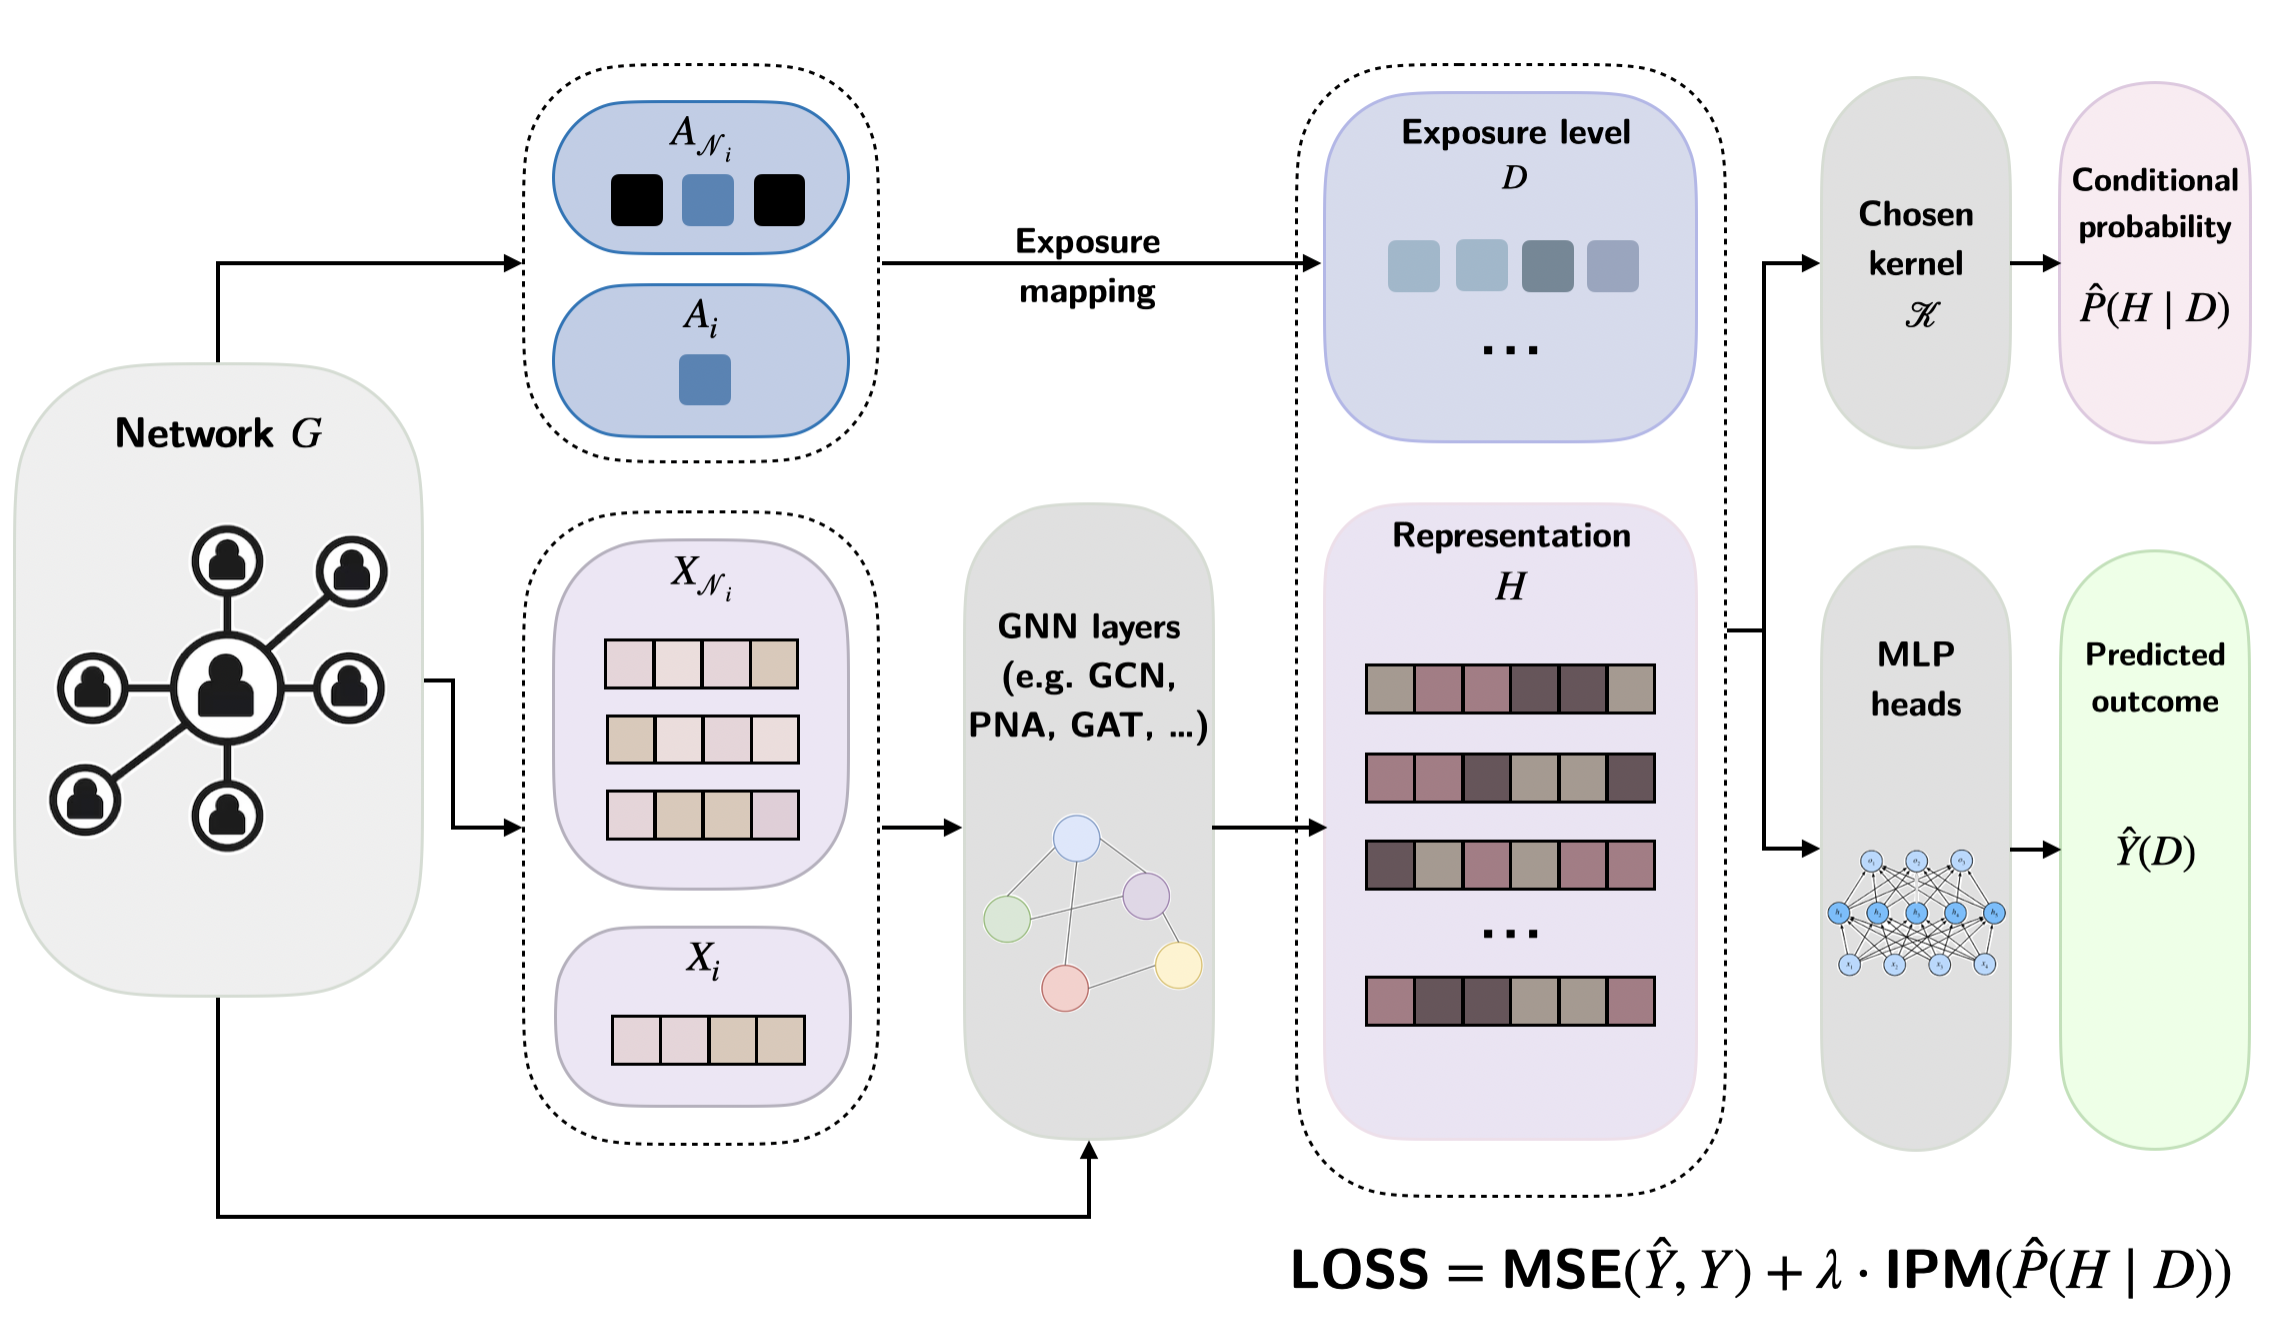
\includegraphics[width=\linewidth]{../architecture.png}
    \caption{Overview of the GNN encoder for potential outcome prediction given exposure mapping. }
    \label{fig:architecture}
\end{figure}

\textbf{Stage 1: Feature extraction.} Given an input graph $\bG$ representing the network structure among $n$ units, we extract both individual-level and neighborhood-level information for each unit $i$. % Specifically, we obtain the individual treatment indicator $A_i$ and covariate vector $X_i$, as well as the treatment indicators $A_{\cN_i} = \{A_j : j \in \cN_i\}$ and covariates $X_{\cN_i} = \{X_j : j \in \cN_i\}$ of unit $i$'s neighbors $\cN_i$. 
The treatment information is aggregated through the exposure mapping to compute the exposure level $D_i$ for each unit, which captures the relevant summary of interference from neighboring units.

\textbf{Stage 2: Representation learning via GNN.} The extracted covariates are processed through multiple layers of Graph Neural Networks (GNNs) to learn informative representations $H = (H_1, \ldots, H_n)^\T$ that encode both individual characteristics and network structure. The GNN layers perform message passing to aggregate information from neighboring nodes, allowing each unit's representation to incorporate relevant contextual information from its local network neighborhood \citep{wu2020comprehensive}. 
The framework is agnostic to the specific GNN architecture and can accommodate various choices.  
% such as Graph Convolutional Networks \citep{kipf2016semi}, Principal Neighbourhood Aggregation \citep{corso2020principal}, or Graph Attention Networks \citep{velivckovic2017graph}. 
See Appendix \ref{sec:gnn_choices} for more details.

\textbf{Stage 3: Outcome prediction and representation balancing.} The learned representations $H$ serve two purposes. First, they are fed into MLP (multilayer perceptron) heads to predict the potential outcomes $\hat{Y}(D)$ at different exposure levels. Second, we employ a chosen kernel $\mathscr{K}$ to estimate the conditional distribution $\hat{{P}}(H \mid D)$ of representations given the exposure level. The model is trained end-to-end using a composite loss function: $
\mathcal{L} = \textup{MSE}(\hat{Y}, Y) + \lambda \cdot \textup{IPM}(\hat{P}(H \mid D)),$ 
where the first term measures the mean squared error of outcome predictions, and the second term penalizes the discrepancy in representation distributions across different exposure levels using an Integral Probability Metric (IPM, \citet{johansson2016learning}), which encourages the learned representations to be balanced across exposure groups.


\subsection{GNN-assisted AIPW estimator}
The above procedure leads to prediction for each unit at each exposure level: $\hat{f}_i^{(d_k)} = \{H_i^{(d_k)}\}{}^\T \hat{\omega}_k,$ $k=1,2,$ 
where $H_i^{(d_k)}$ is the representation for unit $i$ at exposure level $d_k$, which is extracted from the second-to-last layer of the $k$-th MLP head. $\hat{\omega}_k$ is the weight for the second-to-last layer of the $k$-th MLP head. Therefore, this corresponds to taking $F_i^{(d_k)} = H_i^{(d_k)}{}^\T$ and $\hat\beta_k = \hat{\omega}_k$ in \eqref{eq::F-beta}.


% The G-AIPW estimator is then given by:
% \begin{align*}
%     \hat\tau^{(d_1,d_2)}_{\textup{adj}} =& \hat{\mu}^{(d_1)}_{\textup{adj}} - \hat{\mu}^{(d_2)}_{\textup{adj}}.
% \end{align*}
% where for $k=1,2$,
% \begin{align*}
%     \hat{\mu}^{(d_k)}_{\textup{adj}} = \frac{1}{n}\sum_{i=1}^n \frac{\indicator{(D_i=d_k)}(Y_i-\hat{Y}_i^{(d_k)})}{\pi_i^{(d_k)}} + \hat{Y}_i^{(d_k)}. 
% \end{align*}

% However, as we have commented in Section \ref{sec::model_assisted_adjustment}, the above procedure does not target variance reduction of the estimator. In the following section, we discuss how to calibrate the GNN-assisted AIPW estimator to facilitate variance reduction. 


\subsection{Two calibration paradigms for GNN prediction}
Now we apply the GER procedure to improve the GNN-assisted AIPW estimator. We consider two calibration paradigms: (i) calibrating the raw predictions; (ii) calibrating the last-layer weight of the GNN.



\textbf{Paradigm 1: Calibrating the raw predictions.} We can take the features in \eqref{eq::bFaug} directly as the GNN predictions, plus an intercept term:
\begin{align*}
    F_i^{(d_k)} = (1, \{\hat{Y}{}_i^{(d_k)}\}{}^\T)^\T, \quad k=1,2.
\end{align*} 
This shares a similar spirit with the so-called no-harm calibration method \citep{fogarty2018regression} in the nonlinear regression adjustment scenario, but here we focus on resolving the interference structure. In this case, using GER to estimate $\beta^\star$ acts as performing affine transformation to the GNN predictions including some recentering and rescaling, so that the adjustment further facilitates variance reduction.

\textbf{Paradigm 2: Calibrating the last-layer weight of the GNN.} We can take the features in \eqref{eq::bFaug} as the last-layer representation of the GNN, plus an intercept term:
\begin{align*}
    F_i^{(d_k)} = (1, H_i^{(d_k)}{}^\T)^\T, \quad k=1,2.
\end{align*}
In this case, using GER to estimate $\beta^\star$ acts as performing modification to the last-layer weight of the GNN. This generally gives a wider range of flexibility in terms of the calibration than Paradigm 1. Yet it comes with the trade-off of a higher variance due to the additional parameter estimation.

% After calibration with either of the two paradigms, we can construct the calibrated G-AIPW estimator $\hat\tau^{\textup{G-cal}}$ as follows:
% \begin{align*}
%     \hat\tau^{(d_1,d_2)}_{\textup{cal}} = \hat{\mu}^{(d_1)}_{\textup{cal}} - \hat{\mu}^{(d_2)}_{\textup{cal}}.
% \end{align*}
% where for $k=1,2$,
% {\small 
% \begin{align*}
%     \hat{\mu}^{(d_k)}_{\textup{cal}} = \frac{1}{n}\sum_{i=1}^n \frac{\indicator(D_i=d_k)(Y_i-{F_i^{(d_k)}}{}^\T \hat{\beta}_k)}{\pi_i^{(d_k)}} + {F_i^{(d_k)}}{}^\T \hat{\beta}_k. 
% \end{align*}
% }


\section{Numerical studies}
\subsection{Synthetic study}
\label{sec:simulation}

We compare the performance of proposed estimators with various other estimators through Monte Carlo simulations with a data generating process (DGP) that incorporates neighbor covariate spillover effects (see Appendix \ref{sec:dgp_simulation}). 

We compare the following classes of estimators: (i) \emph{Primitive estimators}: Horvitz-Thompson ($\hat\tau^{\hort}$) and H\'{a}jek ($\hat\tau^{\haj}$); (ii) \emph{Linear class}: linear model class based directly on the covariates. (iii)  \emph{GAT class}: Graph Attention Network based methods; (iv) \emph{PNA class}: Principal Neighbourhood Aggregation based methods. For (ii)-(iv), we consider three AIPW estimators each: (i) using raw predictions ($*$-raw); (ii) keeping the covariates or learned representations and calibrating the last linear layer weights ($*$-linear); (iii) calibrating the raw predictions with no-harm calibration ($*$-pred). The GNN-based methods use the architecture described in Section~\ref{sec::g-aipw}, with hyperparameters tuned as described in Section~\ref{sec:hyperparameter_tuning}. 

Table~\ref{tab::simu_results} reports bias, standard deviation (SD), and root mean squared error (RMSE) from $B=30$ Monte Carlo replications, along with 95\% confidence interval coverage and power. The Horvitz-Thompson estimator performs poorly with only 60\% coverage, demonstrating its poor behavior. H\'{a}jek estimator achieves much better behavior in all dimensions. Using raw linear prediction for adjustment leads to similar performance to the H\'{a}jek estimator, and calibrating the raw predictions leads to significant improvement. All three PNA-calibrated estimators achieve the lowest RMSE and perform nearly identically, suggesting that PNA's learned representations are already achieving good balance in prediction accuracy and variance reduction. In contrast, GAT-raw performs worse than GAT-linear and GAT-pred, indicating that GAT predictions benefit more from additional linear calibration.
\begin{table*}[h!]
    \centering
    \caption{Simulation results comparing estimators under DGP with neighbor spillover. True $\tau^\star = -0.594$. Linear model achieves $0.121 \pm 0.006$ $R^2$. GAT achieves $0.327 \pm 0.056$ $R^2$. PNA achieves $0.533 \pm 0.015 $ $R^2$. The $\pm$ indicating radius of a $90\%$ confidence interval across $100$ Monte Carlo simulations. }
    \small
    \begin{tabular}{ll|ccc|cc}
        \toprule
        Description & Estimator & Bias & SD & RMSE & Coverage & Power \\
        \midrule
        Primitive  & $\hat\tau^{\hort}$ & $-0.049 \pm 0.09$ & $0.541 \pm 0.06$ & $0.543 \pm 0.06$ & 0.60 & 0.66 \\
        & $\hat\tau^{\haj}$ & $0.018 \pm 0.03$ & $0.203 \pm 0.02$ & $0.203 \pm 0.02$ & 0.97 & 0.74 \\
        \midrule
        Linear 
        & $\hat\tau^{\textup{linear-raw}}$ & $-0.017 \pm 0.03$ & $0.202 \pm 0.02$ & $0.203 \pm 0.02$ & 0.99 & 0.82 \\
        & $\hat\tau^{\textup{linear-linear}}$ & $0.034 \pm 0.03$ & $0.170 \pm 0.02$ & $0.173 \pm 0.02$ & 0.97 & 0.82 \\
        & $\hat\tau^{\textup{linear-pred}}$ & $0.040 \pm 0.03$ & $0.172 \pm 0.02$ & $0.176 \pm 0.02$ & 0.97 & 0.81 \\
        \midrule
        GAT 
        & $\hat\tau^{\textup{GAT-raw}}$ & $0.035 \pm 0.03$ & $0.168 \pm 0.02$ & $0.172 \pm 0.02$ & 0.96 & 0.89 \\
        & $\hat\tau^{\textup{GAT-linear}}$ & $0.058 \pm 0.02$ & $0.141 \pm 0.02$ & $0.152 \pm 0.02$ & 0.98 & 0.95 \\
        & $\hat\tau^{\textup{GAT-pred}}$ & $0.058 \pm 0.02$ & $0.140 \pm 0.02$ & $0.152 \pm 0.02$ & 0.98 & 0.95 \\
        \midrule
        PNA 
        & $\hat\tau^{\textup{PNA-raw}}$ & $\mathbf{-0.001 \pm 0.02}$ & $\mathbf{0.127 \pm 0.01}$ & $\mathbf{0.127 \pm 0.01}$ & 0.97 & 1.00 \\
        & $\hat\tau^{\textup{PNA-linear}}$ & $\mathbf{0.008 \pm 0.02}$ & $\mathbf{0.125 \pm 0.01}$ & $\mathbf{0.125 \pm 0.01}$ & 0.98 & 1.00 \\
        & $\hat\tau^{\textup{PNA-pred}}$ & $\mathbf{0.009 \pm 0.02}$ & $\mathbf{0.124 \pm 0.01}$ & $\mathbf{0.124 \pm 0.01}$ & 0.98 & 1.00 \\
        \bottomrule
    \end{tabular}
    \label{tab::simu_results}
\end{table*}


\begin{table*}[h!]
    \centering
    \caption{Treatment effect estimates for revenue per enterprise (KES). * denotes statistical significance at $\alpha=0.05$.}
    \label{tab:revenue_results}
    \small
    \begin{tabular}{l cc cc cc cc}
        \toprule
        & \multicolumn{2}{c}{HT} & \multicolumn{2}{c}{H\'{a}jek} & \multicolumn{2}{c}{Linear} & \multicolumn{2}{c}{PNA-no-harm} \\
        \cmidrule(lr){2-3} \cmidrule(lr){4-5} \cmidrule(lr){6-7} \cmidrule(lr){8-9}
        Contrast & $\hat\tau$ & 95\% CI & $\hat\tau$ & 95\% CI & $\hat\tau$ & 95\% CI & $\hat\tau$ & 95\% CI \\
        \midrule
        Direct ($H=0$) & 2786* & [405, 5167] & 841 & [-1085, 2767] & 879 & [-1084, 2842] & 731 & [-1088, 2549] \\
        Direct ($H=1$) & 113 & [-1185, 1410] & 1391* & [105, 2678] & 1356* & [96, 2617] & 1390* & [186, 2594] \\
        Spillover ($A=0$) & 3770* & [1963, 5577] & 46 & [-1372, 1464] & -75 & [-1479, 1329] & -64 & [-1402, 1275] \\
        Spillover ($A=1$) & 1097 & [-774, 2969] & 596 & [-1198, 2390] & 481 & [-1508, 2470] & 536 & [-1215, 2288] \\
        \bottomrule
    \end{tabular}
\end{table*}


% All regression-based methods achieve near-nominal coverage ($\geq 0.96$), with PNA methods achieving perfect power (1.00). Table~\ref{tab::r2_results} reports the outcome prediction $R^2$ for each model class, confirming that PNA learns substantially more predictive representations that capture the neighbor spillover structure in \eqref{eq:dgp_spillover}.

% \begin{table}[h]
%     \centering
%     \caption{Outcome prediction $R^2$ by model class (mean $\pm$ std across MC replications).}
%     \begin{tabular}{l|c}
%         \toprule
%         Model & $R^2$ \\
%         \midrule
%         Linear & $0.121 \pm 0.006$ \\
%         GAT & $0.327 \pm 0.056$ \\
%         PNA & $\mathbf{0.533 \pm 0.015}$ \\
%         \bottomrule
%     \end{tabular}
%     \label{tab::r2_results}
% \end{table}

% The key advantage of PNA over GAT lies in its degree-aware aggregation. While GAT's softmax attention normalizes neighbor contributions regardless of degree, PNA's sum aggregator and degree scalers preserve the neighborhood size information that is essential for capturing the spillover term $\frac{1}{|\cN_i|}\sum_{j \in \cN_i} g(X_j)$. This enables PNA to learn representations that better explain outcome heterogeneity, leading to more effective variance reduction through calibration.


\subsection{Real application}
\label{sec:application}

We apply our GAUGER framework to analyze data from a large-scale randomized controlled trial studying the effects of unconditional cash transfers in rural Kenya \citep{egger2022general}. The GiveDirectly experiment implemented a randomized saturation design across 653 villages in Siaya County, Kenya. In this design, sublocations (administrative units containing multiple villages) were first randomly assigned to either high-saturation (two-thirds of villages treated) or low-saturation (one-third of villages treated) conditions. Within each sublocation, villages were then randomly assigned to treatment or control. All eligible households in treated villages received unconditional cash transfers of approximately \$1,000 USD. We construct a spatial network among villages based on geographic proximity, following our desciption in Appendix \ref{sec:village-network}.

We define the exposure mapping as $D_i = (A_i, S_i)$, where $A_i \in \{0, 1\}$ is the village's own treatment indicator, and $S_i = \indicator({|\cN_i|^{-1}}{\sum_{j \in \cN_i} A_j} > {1}/{3})$ indicates whether more than one-third of village $i$'s neighbors are treated. This yields four exposure levels: $(A_i, S_i) \in \{(0,0), (0,1), (1,0), (1,1)\}$. The exposure $(0,0)$ corresponds to untreated villages with few treated neighbors, while $(1,1)$ corresponds to treated villages with many treated neighbors. The contrast between $(1,0)$ and $(0,0)$ captures the direct effect of treatment with low neighborhood saturation, while $(0,1)$ versus $(0,0)$ captures the spillover effect on untreated villages from having many treated neighbors.






Table~\ref{tab:revenue_results} presents treatment effect estimates for revenue per enterprise (in Kenyan Shillings or KES). The H\'{a}jek, Linear, and PNA-no-harm estimators yield consistent conclusions: a statistically significant positive direct effect when neighbors are mostly treated ($H=1$), with point estimates around 1,356--1,391 KES. In contrast, the Horvitz-Thompson estimator produces misleading results---it shows spurious significance for Direct ($H=0$) and Spillover ($A=0$) due to its sensitivity to extreme inverse probability weights, while missing the true Direct ($H=1$) effect. Table~\ref{tab:revenue_ci_width} presents 95\% confidence interval widths for the treatment effect estimates, showing that the PNA-no-harm estimator achieves the narrowest average confidence interval width for all four contrasts. This efficiency gain comes from the PNA model's ability to leverage network structure for outcome prediction, reducing residual variance.




\section{Discussion}
In this paper, we have proposed a GAUGER framework for estimating treatment effects under interference. We have shown that the GAUGER framework can be used to estimate treatment effects under interference and provide a principled way to construct model adjustment for statistical efficiency. We have also shown that the GAUGER framework can be implemented using GNNs to achieve substantial efficiency gains over existing methods.

There are many remaining questions and extensions to the current work. For example, most exposure mappings are discrete, and it is worth exploring how to extend the GAUGER framework to continuous exposure mappings. Moreover, it is an interesting question to explore how to use GAUGER for facilitating a better experimental design on the networks for better effect estimation. 




% \section*{Accessibility}

% Authors are kindly asked to make their submissions as accessible as possible
% for everyone including people with disabilities and sensory or neurological
% differences. Tips of how to achieve this and what to pay attention to will be
% provided on the conference website \url{http://icml.cc/}.

% \section*{Software and Data}
% Our software and data are uploaded as Supplementary Material to the OpenReview reviewing system.

% If a paper is accepted, we strongly encourage the publication of software and
% data with the camera-ready version of the paper whenever appropriate. This can
% be done by including a URL in the camera-ready copy. However, \textbf{do not}
% include URLs that reveal your institution or identity in your submission for
% review. Instead, provide an anonymous URL or upload the material as
% ``Supplementary Material'' into the OpenReview reviewing system. Note that
% reviewers are not required to look at this material when writing their review.

% Acknowledgements should only appear in the accepted version.
% \section*{Acknowledgements}

% \textbf{Do not} include acknowledgements in the initial version of the paper
% submitted for blind review.

% If a paper is accepted, the final camera-ready version can (and usually should)
% include acknowledgements.  Such acknowledgements should be placed at the end of
% the section, in an unnumbered section that does not count towards the paper
% page limit. Typically, this will include thanks to reviewers who gave useful
% comments, to colleagues who contributed to the ideas, and to funding agencies
% and corporate sponsors that provided financial support.

\section*{Impact Statement}

This paper presents work whose goal is to advance the field of causal inference under interference, using machine learning and deep learning techniques. There are many potential societal consequences of our work, none which we feel must be specifically highlighted here.

% Authors are \textbf{required} to include a statement of the potential broader
% impact of their work, including its ethical aspects and future societal
% consequences. This statement should be in an unnumbered section at the end of
% the paper (co-located with Acknowledgements -- the two may appear in either
% order, but both must be before References), and does not count toward the paper
% page limit. In many cases, where the ethical impacts and expected societal
% implications are those that are well established when advancing the field of
% Machine Learning, substantial discussion is not required, and a simple
% statement such as the following will suffice:

% ``This paper presents work whose goal is to advance the field of Machine
% Learning. There are many potential societal consequences of our work, none
% which we feel must be specifically highlighted here.''

% The above statement can be used verbatim in such cases, but we encourage
% authors to think about whether there is content which does warrant further
% discussion, as this statement will be apparent if the paper is later flagged
% for ethics review.

% In the unusual situation where you want a paper to appear in the
% references without citing it in the main text, use \nocite
% \nocite{langley00}



\bibliography{example_paper}
\bibliographystyle{icml2026}

%%%%%%%%%%%%%%%%%%%%%%%%%%%%%%%%%%%%%%%%%%%%%%%%%%%%%%%%%%%%%%%%%%%%%%%%%%%%%%%
%%%%%%%%%%%%%%%%%%%%%%%%%%%%%%%%%%%%%%%%%%%%%%%%%%%%%%%%%%%%%%%%%%%%%%%%%%%%%%%
% APPENDIX
%%%%%%%%%%%%%%%%%%%%%%%%%%%%%%%%%%%%%%%%%%%%%%%%%%%%%%%%%%%%%%%%%%%%%%%%%%%%%%%
%%%%%%%%%%%%%%%%%%%%%%%%%%%%%%%%%%%%%%%%%%%%%%%%%%%%%%%%%%%%%%%%%%%%%%%%%%%%%%%
\newpage
\appendix
\onecolumn

\section{Additional details}
\subsection{Monte Carlo approximation for $\bLambda$}\label{sec:mc_lambda}
One key step for the framework is to perform Monte Carlo approximation to estimate the matrix $\bLambda$. We use the Monte Carlo simulation approach introduced by Section 3 of \citet{aronow2017estimating}. Introduce the following matrix $\bPi^{(d_k,d_l)}\in\mathbb{R}^{n\times n}$ to encode the probabailities in \eqref{eq::prob-d} and \eqref{eq::prob-dd}, with elements:
\begin{align}
    \{\bPi^{(d_k, d_l)}\}_{ij} =
    \left\{
        \begin{array}{ll}
            \pi_i^{(d_k)}, & i=j,~ k=l;\\
            \pi_{ij}^{(d_k, d_l)}, & \text{otherwise}.
        \end{array}
    \right.
\end{align}
Based on \eqref{eq::bLambda}, $\bLambda$ can be directly computed from $\bPi^{(d_k, d_l)}$. Algorithm \ref{alg:MC_Lambda} summarizes the procedure to compute $\bLambda$. 
\begin{algorithm}[ht!]
    \caption{Monte Carlo Simulation for Computing $\bLambda^{(d_k, d_l)}$}
    \label{alg:MC_Lambda} 
 \begin{algorithmic}[1]
    \STATE {\bfseries Input:} Randomization plan $\mathcal{P}$, rounds of Monte Carlo repetition $R$, number of exposure levels $K$, number of unites $n$, network $\bG$ 
 %   \REPEAT
    \STATE Perform $R$ rounds of randomization following $\mathcal{P}$, to construct $K$ indicator-of-exposure matrix in $\{0,1\}^{n\times R}$, given by 
    $
    \mathbbm{1}^{\textup{MC}}_k = \{1^{(r)}(D_i = d_k)\}_{i\in[n], r\in[R]}, 
    $
    where $1^{(r)}(D_i = d_k)$ indicates whether unit $i$ has exposure level $d_k (k=1,2)$ in Round $r$.

    \FOR{k=1,2} 
    \STATE Compute $\hat\bPi{}^{(d_k,d_k)} = \{\mathbbm{1}^{\textup{MC}}_k \cdot (\mathbbm{1}^{\textup{MC}}_k)^\T + I_n\}/(R+1)$. The $(i,i)$-th diagonal of $\hat\bPi{}^{(d_k,d_k)}$ approximates the propensity scores $\pi_i^{(d_k)}$, and the $(i,j)$-th off-diagonal value approximates the joint inclusion probability $\pi_{ij}^{(d_k,d_k)}$. 
    \ENDFOR
    
    % \FOR{$k=1,\cdots, K-1$}
    % \FOR{$j = k+1, \cdots, K$}
    % \STATE Compute $\hat\Pi(d_k,d_l) = \{\mathbbm{1}^{\textup{MC}}_k \cdot (\mathbbm{1}^{\textup{MC}}_l)^\T\}/R$. The $(i,j)$-th value approximates the joint inclusion probability $\pi_{ij}(d_k,d_l)$. 
    % \ENDFOR
    % \ENDFOR
    \STATE Compute $\hat\bPi{}^{(d_k,d_l)} = \{\mathbbm{1}^{\textup{MC}}_k \cdot (\mathbbm{1}^{\textup{MC}}_l)^\T\}/R$. The $(i,j)$-th value approximates the joint inclusion probability $\pi_{ij}^{(d_k,d_l)}$.
     
    \STATE Use the definition \eqref{eq::bLambda} to construct $\hat\bLambda^{(d_k,d_l)}$ from $\hat\bPi^{(d_k,d_l)}$. 
    \STATE \textbf{Output: }  $\hat\bLambda{}^{(d_k,d_l)}$ and $\hat\bPi{}^{(d_k,d_l)}$.
 %  \UNTIL{$noChange$ is $true$}
 \end{algorithmic}
 \end{algorithm}

\citet{aronow2017estimating} also provides a theoretical justification for Algorithm \ref{alg:MC_Lambda}, which suggests that the Monte Carlo approximation is asymptotically consistent:
\begin{proposition}[Proposition 3.1 in \citet{aronow2017estimating}]
    As $R \rightarrow \infty$, $\hat{\bPi}{}^{(d_k,d_l)} \rightarrow \bPi^{(d_k,d_l)}$ almost surely. Thus, we also have that $\hat\bLambda{}^{(d_k,d_l)} \rightarrow \bLambda^{(d_k,d_l)}$ almost surely.
\end{proposition}

\begin{remark}[Computational complexity of Algorithm \ref{alg:MC_Lambda}]\label{remark:mc_lambda}
    The main computational cost of Algorithm \ref{alg:MC_Lambda} is the computation of the matrix $\hat\bPi{}^{(d_k,d_l)}$, which requires $O(n^2R)$ operations. More broadly, if we apply Algorithm \ref{alg:MC_Lambda} to compute the matrix $\bLambda$ for $K$ exposure levels, the computational complexity is $O(n^2K^2R)$.
\end{remark}

\subsection{Variance estimation}\label{sec:variance_estimation}
Following the tradition of design-based inference, it is not possible to construct a consistent variance estimator for $\hat\tau^{(d_1, d_2)}_{F, \hat\beta}$, because we can never observe and estimate the cross-level covariance between potential outcomes. Instead, we need to construct a variance estimator with a certain level of conservativeness to be robust to different possible cross-level correlations. 

First, we define the following matrix:
\begin{align*}
    \bPhi_{kl} = \textup{diag}\{\phi_{i+}^{(d_k, d_l)}\}_{i=1}^n, \quad k = 1,2, 
\end{align*}
where $\phi_{i+}^{(d_k, d_l)} = \sumj \indicator(\pi_{ij}^{(d_k, d_l)} = 0, \bDelta_{ij} = 1) $ counts the number of units $j$ under level $d_l$ that have $D_j \nonindep D_i$ and are never jointly included in the sample with $i$ under exposure $d_k$. The reweighted version is given by
\begin{align*}
    \bPhi_{kl}^\pi = \textup{diag}\{\pi_i^{(d_k)}\phi_{i+}^{(d_k, d_l)}\}_{i=1}^n,
\end{align*}

Then, we define the following matrix, which is a augmented version of $\bLambda$: 
\begin{eqnarray*}
    \{\bLambda_{kl}^\pi\}_{(i,j)}
    =  
    \left\{
        \begin{array}{cc}
            \{\bLambda_{kl}\}_{(i,j)} \cdot \frac{\pi_i^{(d_k)}\pi_i^{(d_l)}}{\pi_{ij}^{(d_k,d_l)}}, & \pi_{ij}^{(d_k,d_l)} \neq 0; \\
            0, & \pi_{ij}(d_k,d_l) = 0. 
        \end{array}
    \right.    
\end{eqnarray*}    
Meanwhile, we construct the following variance estimator:
\begin{align}\label{eq::var_est}
    \hat{v}^{(d_1,d_2)} = \left(
        \sqrt{\hat{v}^{(d_1)}} + \sqrt{\hat{v}^{(d_2)}}
    \right)^2,
\end{align}
where for $k = 1,2$,
{\small 
\begin{align*}
    &\hat{v}^{(d_k)} = n^{-2} \{\hat{\bY}{}^{(d_k)} - \hat{\bF}{}^{(d_k)}\hat\beta_k\}^\T (\bLambda_{kk}^\pi + \bPhi_{kk}^\pi) \{\hat{\bY}{}^{(d_k)} - \hat{\bF}{}^{(d_k)}\hat\beta_k\}. 
\end{align*}
}
The variance estimator motivates the following confidence interval:
\begin{align*}
    \hat\tau^{(d_1,d_2)}_{F, \hat{\beta}} \pm z_{\alpha/2} \sqrt{\hat{v}^{(d_1,d_2)}},
\end{align*}
where $z_{\alpha/2}$ is the $1-\alpha/2$ quantile of the standard normal distribution.


The following theorem shows the conservativeness of the variance estimator $\hat{v}(d_1,d_2)$.
\begin{theorem}[Conservative variance estimator and CI]\label{thm:var_est}
    Assume Assumption \ref{asp::positivity_a}-\ref{asp::stability}, and a consistent estimator $\hat\beta$ of $\beta^\star$, i.e., $\hat\beta - \beta^\star = o_p(1)$. Define 
    \begin{eqnarray*} 
        v_{\lim}^{(d_1, d_2)} = \left\{\sqrt{v_{\lim}^{(d_1)}} + \sqrt{v_{\lim}^{(d_2)}}\right\}^2, 
    \end{eqnarray*}
    where $v_{\lim}^{(d_k)}$ is given in Appendix \ref{sec:pf-var-est}.   
    % {\small
    % \begin{eqnarray*}
    %     v_{\lim}^{(d_k)} = (\bY^{(d_k)}-\bF^{(d_k)}\beta^\star)^{\T} (\bLambda_{kk}^+ + \bPhi_{kk}^+) (\bY^{(d_k)}-\bF^{(d_k)}\beta^\star). 
    % \end{eqnarray*}
    % }
    % {\color{blue} i guess it is not $\bLambda_{kk}^+ + \bPhi_{kk}^+$ but $\pi$ as superscript.}
    Then the variance estimator \eqref{eq::var_est} is conservative:
    \begin{eqnarray*}
        \frac{\hat{v}^{(d_1,d_2)} - v_{\lim}^{(d_1,d_2)}}{v_{\lim}^{(d_1,d_2)}} = o_p(1), \quad v_{\lim}^{(d_1,d_2)} \ge \avar\{\hat\tau^{(d_1,d_2)}_{F, \hat\beta}\}.
    \end{eqnarray*}
\end{theorem}
The conservativeness of the variance estimator also guarantees the validity of the confidence interval. 

\subsection{Computation complexity for hyperparameter construction}\label{sec:computation}

In this section, we comment on the computation complexity of the hyperparameter construction, when there are $K$ pairs of contrast exposures we want to compare.

Applying GER to estimate $\beta^\star$ only requires computation of $\bDelta$ and the first-order inclusion probabilities \eqref{eq::prob-d}, and there is no need for the second-order inclusion probabilities \eqref{eq::prob-dd}. This improves the computation complexity to $O(nKR)$ for first-order inclusion probabilities where $R$ is the number of rounds of Monte Carlo simulation, plus $O(n \delta_n^2)$ for constructing $\bDelta$, resulting in a total computational complexity of $O(nKR + n \delta_n^2)$ for hyperparameter construction.

Another straightforward approach is to estimate $\beta^\star$ by a plug-in approach using IPW counterpart for $\bY^{(d_1;d_2)}$, as well as $\bFaug$. Such an approach has been discussed in multiple literature for design-based causal inference, such as \citet{middleton2018unified, chang2023design, lu2025design}. Based on our discussion in Appendix \ref{sec:mc_lambda}, when there are $K$ pairs of contrast exposures, the computational complexity is $O(K n^2 R)$, where $R$ is the number of rounds of Monte Carlo simulation. 

\subsection{Choice of GNN architecture}\label{sec:gnn_choices}

Our framework is agnostic to the specific GNN architecture. We describe common choices following the message-passing paradigm where unit $i$'s representation $H_i^{(\ell)}$ at layer $\ell$ is updated by aggregating from neighbors $\cN_i$. Let $H_i^{(0)} = X_i$.

\begin{enumerate}[leftmargin=*]
    \item \textbf{GCN} \citep{kipf2016semi}: Normalized mean aggregation. $H_i^{(\ell+1)} = \sigma\big( W^{(\ell)} \cdot \frac{1}{|\cN_i|+1} ( H_i^{(\ell)} + \sum_{j \in \cN_i} \frac{H_j^{(\ell)}}{\sqrt{|\cN_j|+1}} ) \big)$. Efficient but treats all neighbors equally.
    
    \item \textbf{GAT} \citep{velivckovic2017graph}: Learned attention weights. $H_i^{(\ell+1)} = \sigma\big( \sum_{j \in \cN_i \cup \{i\}} \alpha_{ij}^{(\ell)} W^{(\ell)} H_j^{(\ell)} \big)$, where $\alpha_{ij}$ are softmax-normalized attention scores computed from node pairs. Focuses on informative neighbors.
    
    \item \textbf{GIN} \citep{xu2018powerful}: Maximally expressive. $H_i^{(\ell+1)} = \textup{MLP}^{(\ell)}\big( (1 + \epsilon^{(\ell)}) H_i^{(\ell)} + \sum_{j \in \cN_i} H_j^{(\ell)} \big)$. Sum aggregation with MLP distinguishes more graph structures.
    
    \item \textbf{PNA} \citep{corso2020principal}: Multiple aggregators with degree scalers. $H_i^{(\ell+1)} = U^{(\ell)} \big( H_i^{(\ell)}, \bigoplus_{\textup{agg}, s} s(|\cN_i|) \cdot \textup{agg}(\{H_j^{(\ell)}\}_{j \in \cN_i}) \big)$, where $\textup{agg} \in \{\textup{mean}, \textup{max}, \textup{min}, \textup{std}\}$ and $s \in \{1, |\cN_i|^{-1/2}, |\cN_i|^{-1}\}$. Robust across different graph types.
\end{enumerate}



\subsection{A cross-fitting extension}\label{sec:cf}

Cross-fitting is a standard technique to reduce overfitting bias when the same data is used for both model fitting and estimation \citep{lu2025conditional}. Under network interference, the dependency structure requires a more careful sample splitting strategy. We propose a graph-based cross-fitting procedure tailored to interference settings, summarized in Algorithm \ref{alg:cross_fitting}.

\begin{algorithm}[ht!]
    \caption{Graph-Based Cross-Fitting for Network Interference}
    \label{alg:cross_fitting}
\begin{algorithmic}[1]
    \STATE {\bfseries Input:} Network $\bG$, covariates $\bX$, outcomes $\bY$, exposures $D_1,\ldots,D_n$, propensities $\pi_i^{(d)}$, balance tolerance $\epsilon > 0$
    
    \STATE \textbf{(Construct 2-hop graph)} Compute $\bG^{(2)}$ where $\bG^{(2)}_{ij} = 1$ if $\cN_i \cap \cN_j \neq \emptyset$ (i.e., units $i$ and $j$ share a common neighbor in $G$).
    
    \STATE \textbf{(Balanced min-cut)} Partition units into $\mathcal{V}_1, \mathcal{V}_2$ by solving:
    $
    \min_{\mathcal{V}_1, \mathcal{V}_2} |\{(i,j) : G^{(2)}_{ij} = 1, i \in \mathcal{V}_1, j \in \mathcal{V}_2\}| ~ \text{s.t.} ~ ||\mathcal{V}_1| - |\mathcal{V}_2|| \leq \epsilon n.
    $
    
    \STATE \textbf{(Create buffer zones)} Define training sets by removing boundary units:
    $\mathcal{T}_1 = \mathcal{V}_1 \setminus \{i : \exists j \in \mathcal{V}_2 \text{ with } G^{(2)}_{ij} = 1\}$, and
    $\mathcal{T}_2 = \mathcal{V}_2 \setminus \{i : \exists j \in \mathcal{V}_1 \text{ with } G^{(2)}_{ij} = 1\}$.
    
    \STATE \textbf{(Fit models)} Train outcome model $\hat{f}_1$ on units in $\mathcal{T}_1$; train $\hat{f}_2$ on units in $\mathcal{T}_2$.
    
    \STATE \textbf{(Cross-predict)} For each unit $i$ and exposure level $d$, compute:
    $
    \hat{Y}_i^{(d),\textup{cf}} = \hat{f}_2(X_i, G; d) \cdot \indicator(i \in \mathcal{V}_1) + \hat{f}_1(X_i, G; d) \cdot \indicator(i \in \mathcal{V}_2).
    $
    
    \STATE \textbf{(Construct estimator)} Compute the cross-fitted AIPW estimator:
    $
    \hat{\mu}^{(d)}_{\textup{cf}} = \frac{1}{n}\sumi \left\{ \frac{\indicator(D_i=d)(Y_i - \hat{Y}_i^{(d),\textup{cf}})}{\pi_i^{(d)}} + \hat{Y}_i^{(d),\textup{cf}} \right\}.
    $
    
    \STATE \textbf{Output:} Cross-fitted estimator $\hat{\tau}^{(d_1,d_2)}_{\textup{cf}} = \hat{\mu}^{(d_1)}_{\textup{cf}} - \hat{\mu}^{(d_2)}_{\textup{cf}}$.
\end{algorithmic}
\end{algorithm}

The key insight is that units in $\mathcal{T}_1$ have no 2-hop neighbors in $\mathcal{V}_2$ (and vice versa), ensuring that each unit's predicted outcome comes from a model trained on independent data. The balanced min-cut in Step 3 can be solved using spectral partitioning \citep{fiedler1973algebraic} or the Kernighan-Lin algorithm \citep{kernighan1970efficient}.  




\subsection{More on exposure mappings}\label{sec:exposure_mapping}

\subsubsection{Choices of exposure mappings}

In this section, we discuss some common choices of exposure mappings. 
\begin{example}[SUTVA baseline]
    One common choice is to use the SUTVA baseline, which is assuming there is no interference, and setting $D_i = A_i$. However, this is often unrealistic in practice as it ignores the possibility of spillover effects.
\end{example}

\begin{example}[Total number of treated neighbors]
    One choice is to use the total number of treated neighbors, coupled with a self-treatment indicator, which is given by $D_i = (\sumj \bG_{ij}A_j, A_i)$. This is a continuous exposure mapping, and it is more sensitive to the number of treated neighbors. However, it might be hard to estimate the spillover effect for certain contrasts given that if certain units have a lot of neighbors. 
\end{example}

\begin{example}[Indicator of whether any neighbor is treated]
    One choice is to use the indicator of whether any neighbor is treated, coupled with a self-treatment indicator, which is given by $D_i = (A_i, \indicator{\exists j \in \cN_i : A_j = 1})$. The indicator gives a binary level of spillover, and it is easy to interpret. However, it is not very sensitive to the number of treated neighbors.
\end{example}

\begin{example}[Exposure bins]
    Another common choice is to use exposure bins, Discretize neighbor summary into levels to define a small set of exposures: $S_i \in \{0,1,2,3+\}$, or quantile bins of treated-neighbor proportion. This is a discrete exposure mapping, and it is easy to interpret. 
\end{example}

\subsubsection{Parameter interpretation with misspecified exposure mappings}

We can also follow the framework of \citet{leung2022causal} and allow for misspecified exposure mappings: $D_i$ need not correctly capture how others affect an individual’s potential
outcome. With the potential outcomes $Y_i(\ba)$, we can define the unit $i$'s expected response
under exposure mapping value $d$ as
\begin{align*}
    \mu_i(d) = \sum_{\ba' \in \{0,1\}^n} Y_i(\ba') P(D = \ba' | T = d).
\end{align*}
which equals the expected potential outcome of unit $i$ over all possible treatment assignment vectors given the exposure mapping value at $d$. Let $\mu(d) = n^{-1} \sumi \mu_i(d)$ be the finite population average and $\mu = (\mu(d) : d \in \cD)$ be the $K\times 1$ vector containing all the $\mu(d)$'s corresponding to exposure mapping values. Our focus will be on contrasting these aggregated avarege potential outcomes. 

\subsubsection{Learning exposure mappings via GNNs}
In many applications, the exposure mapping is not known a priori. We propose a data-driven approach to learn the exposure mapping using GNNs. The key idea is to learn a categorical representation that captures how a unit's own treatment and its neighbors' treatments jointly affect the outcome.

\begin{enumerate}[leftmargin=*]
    \item \textbf{Covariate encoding.} Encode pretreatment covariates and network structure: $\phi_i = \textup{GNN}_X(G, \bX)_i$, where $\phi_i \in \mathbb{R}^{d_\phi}$ captures unit $i$'s covariates and local network structure.
    
    \item \textbf{Treatment encoding.} Encode the treatment assignment pattern via a separate GNN: $\psi_i = \textup{GNN}_A(G, \bA)_i$, where $\psi_i \in \mathbb{R}^{d_\psi}$ captures how unit $i$'s own treatment and its neighbors' treatments jointly determine the exposure.
    
    \item \textbf{Exposure categorization.} Pass the treatment encoding through a softmax layer: $\pi_i = \textup{softmax}(W \psi_i)$, where $W \in \mathbb{R}^{K \times d_\psi}$ and $K$ is the number of exposure categories. The discrete exposure is $D_i = \argmax_k \{\pi_{i,k}\}$.
    
    \item \textbf{Gumbel-softmax relaxation.} Since $\argmax$ is non-differentiable, we use the Gumbel-softmax trick \citep{jang2016categorical, maddison2016concrete} during training:
    \begin{align*}
        e_i = \textup{softmax}\left(\frac{\log \pi_i + g_i}{\tau}\right),
    \end{align*}
    where $g_i$ contains i.i.d.\ Gumbel(0,1) samples and $\tau > 0$ is a temperature parameter annealed during training.
    
    \item \textbf{Outcome model and loss.} The outcome model is $\hat{Y}_i = f(\phi_i, e_i; \theta)$, trained by minimizing:
    \begin{align}\label{eq::learned_exposure_loss}
        \mathcal{L} = \underbrace{\frac{1}{n}\sumi (Y_i - \hat{Y}_i)^2}_{\text{MSE loss}} + \lambda \cdot \underbrace{\textup{IPM}(\{\phi_i\}_{D_i=d}, \{\phi_i\}_{D_i=d^{\prime}})}_{\text{Balance loss}},
    \end{align}
    where the IPM loss (e.g., MMD or Wasserstein distance) encourages balanced representations across exposure groups.
\end{enumerate}

At inference time, we use the hard assignment $D_i = \argmax_k \{\pi_{i,k}\}$ to obtain discrete exposure categories for use in our GAUGER framework.




\section{Additional Theoretical Results}
In this section, we provide additional theoretical results. They serve as intermediate steps in the proofs of the main results, but also stand alone as insights on the general properties of the proposed framework. Let's define $\hat\tau{}^{(d_1, d_2)}_{\beta^*}$ as the AIPW estimator \eqref{eq::aipw_def} with a given set of features and the optimal oracle coefficients $\beta^*$ from \eqref{eq::beta-star}. The following theorem shows the consistency of $\hat\tau{}^{(d_1, d_2)}_{\beta^*}$.
\begin{theorem}[Consistency of the linearly adjusted estimator]\label{thm:consistency}
    Under Assumption \ref{asp::positivity_a}-\ref{asp::stability}, the variance of the linearly adjusted estimator has the order:
    \begin{eqnarray}\label{eq::variance_rate}
        \var\{\hat\tau{}^{(d_1, d_2)}_{\beta^*}\} = \Theta\left(\frac{\kappa_n}{n}\right).
    \end{eqnarray}
    Therefore, the linearly adjusted estimator is consistent under the scaling $\kappa_n = o(n)$:
    \begin{align*}
        \hat\tau{}^{(d_1, d_2)}_{\beta^*} - \tau^{(d_1, d_2)} = O_{p}\left(\sqrt{\frac{\kappa_n}{n}}\right) = o_p(1). 
    \end{align*}
    
\end{theorem}


Below we prove asymptotic normality of the AIPW estimator with the oracle coefficients $\beta^*$. 
% We will use a result from \cite{chen2004normal}. For self-consistency, we include the following lemma for CLT under graph dependency. Consider a set of random variables $\{V_i, i \in \mathcal{V}\}$ indexed by the vertices
% of a graph $\mathcal{G} = (\mathcal{V}, \mathcal{E})$. $\mathcal{G}$ is said to be a dependency graph if, for any pair of disjoint sets $\Gamma_1$ and $\Gamma_2$ in $\mathcal{V}$ such that no edge in $\mathcal{E}$ has one endpoint in $\Gamma_1$ and the other in $\Gamma_2$, the sets of random variables $\{V_i, i \in \Gamma_1\}$ and $\{V_i, i \in \Gamma_2\}$ are independent. Let $D$ denote the maximal degree of $\mathcal{G}$, that is, the maximal number of edges incident to a single vertex.
% \begin{lemma}[A CLT under graph dependency, Theorem 2.7 in \cite{chen2004normal}]\label{lem::clt_graph_dependency}
%     Let $\{V_i, i \in \mathcal{V}\}$ be random variables indexed by the vertices of a dependency graph $\mathcal{G} = (\mathcal{V}, \mathcal{E})$. Put $W = \sumi V_i$. Assume that $\E(W^2) = 1$, $\E(V_i) = 0$ and $\E(|V_i|^p) \leq \theta^p$ for $i \in \mathcal{V}$ and for some $2 < p \le 3$ and $\theta > 0$. Then for any $z\in\mathbb{R}$,
%     \begin{eqnarray*}
%         |P(W \leq z) - \Phi(z)| \leq 75 D^{5(p-1)}|V|\theta^p. 
%     \end{eqnarray*}
% \end{lemma}
\begin{theorem}[Asymptotic normality of the linearly adjusted estimator]\label{thm:normality-app}
    Under Assumption \ref{asp::positivity_a}-\ref{asp::stability}, we have the following Berry-Esseen bound:
    \begin{align*}
        \left|P\left(\frac{\hat\tau{}^{(d_1, d_2)}_{\beta^*} - \tau^{(d_1, d_2)}}{\sqrt{\var\{\hat\tau{}^{(d_1, d_2)}_{\beta^*}\}}} \leq z\right) - \Phi(z)\right| \leq \frac{C M_n^3 \delta_n^{20} \eta_n^3}{n^{1/2} \kappa_n^{3/2} },
    \end{align*}
    where $C$ is a constant. Therefore, the linearly adjusted estimator is asymptotically normal:
    \begin{align*}
       \frac{\hat\tau{}^{(d_1, d_2)}_{\beta^*} - \tau^{(d_1, d_2)}}{\sqrt{\var\{\hat\tau{}^{(d_1, d_2)}_{\beta^*}\}}} \rightarrow \cN(0, 1).
    \end{align*}
\end{theorem}
Theorem \ref{thm:normality} provides the asymptotic distribution of the estimator. It builds the foundation of confidence interval construction. The Berry-Esseen bound is of independent interest as an addition to finite-population distribution approximation theory \citep{shi2025berry,Masoero2026multiple}.



Now we need to move to consider the estimator with a plug-in coefficient, as we can never implement the AIPW estimator with an oracle coefficient:
\begin{eqnarray*}
    \hat\tau{}^{(d_1, d_2)}_{\hat\beta} &=& \hat\mu{}^{(d_1)}_{\hat\beta_1} - \hat\mu{}^{(d_2)}_{\hat\beta_2},
\end{eqnarray*}
where, for $k \in \{1,2\}$,
\begin{eqnarray*}
    \hat\mu^{(d_k)}_{\hat\beta} &=& n^{-1}\sumi\frac{\indicator(D_i=d_k)(Y_i-F_i^{(d_k)\T} \hat\beta_k)}{\pi_i^{(d_k)}} + F_i^{(d_k)\T} \hat\beta_k.
\end{eqnarray*}
with $\hat\beta_1$ and $\hat\beta_2$ being the plug-in coefficients.  
\begin{theorem}[Properties with a plug-in coefficient]\label{thm:plug_in}
    Under Assumption \ref{asp::positivity_a}-\ref{asp::stability}, and assume that $\hat\beta$ is consistent, i.e., $\hat\beta - \beta^\star = o_p(1)$. The plug-in coefficient estimator is asymptotically normal as $n\to\infty$:
    \begin{eqnarray*}
        \frac{\hat\tau^{\textup{adj}}_{\hat{\beta}} - \tau}{\sqrt{\avar\{\hat\tau^{\textup{adj}}_{\hat\beta}\}}} \rightarrow \cN(0, 1).
    \end{eqnarray*}
\end{theorem}
Theorem \ref{thm:plug_in} is a strong result stating that the plug-in AIPW estimator also enjoys the asymptotic normality, as long as the estimated coefficient is consistent. Hence, the focus of the problem goes to verifying the GER procedure from \eqref{eq::regression} gives a consistent estimator to the oracle $\beta^\star$. This is established by Theorem \ref{thm:convergence_beta}. 


  

% \begin{theorem}[Conservative variance estimator and CI]\label{thm:var_est}
%     Assume Assumption \ref{asp::positivity}, \ref{asp::bound}, \ref{asp::bounded_degree}, \ref{asp::pop_cov}, and a consistent estimator $\hat\beta$ of $\beta^\star$, i.e., $\hat\beta - \beta^\star = o_p(1)$. Define 
%     \begin{eqnarray*} 
%         v_{\lim} = \{\sqrt{v_{\lim}(d_1)} + \sqrt{v_{\lim}(d_2)}\}^2, 
%     \end{eqnarray*}
%     where     
%     \begin{eqnarray*}
%         v_{\lim}(d_k) = (\bY(d_k)-\bX\beta^\star)^{\T} (\bLambda_{kk}^+ + \bPhi_{kk}^+) (\bY(d_k)-\bX\beta^\star). 
%     \end{eqnarray*}
%     Then the variance estimator \eqref{eq::var_est} is conservative:
%     \begin{eqnarray*}
%         \frac{\hat{v} - v_{\lim}}{v_{\lim}} = o_p(1), \quad v_{\lim} \ge \var(\hat\tau^{\textup{adj}}_*).
%     \end{eqnarray*}
% \end{theorem}


\section{Proof}\label{sec:proof}
\subsection{Proof of Theorem \ref{thm:mean_variance}}
\begin{proof}
    First, we have that
    \begin{eqnarray*}
        \E\{(Y_i - F_i^{(d_k)\T} \beta_k)\indicator(D_i=d_k)/\pi_i^{(d_k)}\} = Y_i^{(d_k)} - F_i^{(d_k)\T} \beta_k.
    \end{eqnarray*}
    Taking a sum over all units, we have that
    \begin{eqnarray*}
        \E\{\hat\mu{}^{(d_1)}_{\beta_1}\} = n^{-1} \sumi Y_i^{(d_1)} - n^{-1} \sumi F_i^{(d_1)\T} \beta_1 + n^{-1} \sumi F_i^{(d_1)\T} \beta_1 = \mu^{(d_1)}, \\
        \E\{\hat\mu{}^{(d_2)}_{\beta_2}\} = n^{-1} \sumi Y_i^{(d_2)} - n^{-1} \sumi F_i^{(d_2)\T} \beta_2 + n^{-1} \sumi F_i^{(d_2)\T} \beta_2 = \mu^{(d_2)}.
    \end{eqnarray*} 
    Thus for any $\beta$, we have that
    \begin{eqnarray*}
        \E\{\hat\tau^{(d_1, d_2)}_{\beta}\} = \E\{\hat\mu^{(d_1)}_{\beta_1}\} - \E\{\hat\mu^{(d_2)}_{\beta_2}\} = \tau^{(d_1, d_2)}.
    \end{eqnarray*}

    For variance, because the only random component in the estimators is the exposure levels $D_i$. For unit $i$, we have:
    \begin{eqnarray*}
        \cov(\indicator(D_i=d), \indicator(D_i=d)) &=& \E(\indicator(D_i=d) \cdot \indicator(D_i=d)) - \E(\indicator(D_i=d)) \cdot \E(\indicator(D_i=d)) \\
        &=& \pi_i^{(d)}(1 - \pi_i^{(d)}), \\
        \cov(\indicator(D_i=d_1), \indicator(D_i=d_2)) &=& \E(\indicator(D_i=d_1) \cdot \indicator(D_i=d_2)) - \E(\indicator(D_i=d_1)) \cdot \E(\indicator(D_i=d_2)) \\
        &=& 0 - \pi_i^{(d_1)}\pi_i^{(d_2)} = - \pi_i^{(d_1)}\pi_i^{(d_2)}, \quad \text{for } d_1\neq d_2.   
    \end{eqnarray*}    
    For two units $i$ and $j$, we have:
    \begin{eqnarray*}
        \cov(\indicator(D_i=d), \indicator(D_j=d)) &=& \E(\indicator(D_i=d) \cdot \indicator(D_j=d)) - \E(\indicator(D_i=d)) \cdot \E(\indicator(D_j=d)) \\
        &=& \pi_{ij}^{(d,d)} - \pi_i^{(d)}\pi_j^{(d)}, \\
        \cov(\indicator(D_i=d_1), \indicator(D_j=d_2)) &=& \pi_{ij}^{(d_1,d_2)} - \pi_i^{(d_1)}\pi_j^{(d_2)} . 
    \end{eqnarray*}    
    The variance of $\hat\tau^{(d_1, d_2)}_{\beta}$ consists of three parts:
    \begin{eqnarray*}
        \var\{\hat\tau^{(d_1, d_2)}_{\beta}\} &=& \var\{\hat\mu^{(d_1)}_{\beta_1}\} + \var\{\hat\mu^{(d_2)}_{\beta_2}\} - 2\cov\{\hat\mu^{(d_1)}_{\beta_1}, \hat\mu^{(d_2)}_{\beta_2}\}.
    \end{eqnarray*}
    For $\var\{\hat\mu^{(d_1)}_{\beta_1}\}$, we have:
    \begin{eqnarray*}
        \var\{\hat\mu^{(d_1)}_{\beta_1}\} &=& \var\left(\frac{1}{n}\sumi \left\{ \frac{\indicator(D_i=d_1)(Y_i-F_i^{(d_1)\T} \beta_1)}{\pi_i^{(d_1)}} + F_i^{(d_1)\T}\beta_1 \right\}\right) \\
        &=& \var\left(\frac{1}{n}\sumi \left\{ \frac{\indicator(D_i=d_1)(Y_i-F_i^{(d_1)\T} \beta_1)}{\pi_i^{(d_1)}} \right\}\right)\\
        &=& \frac{1}{n^2} \sumi \frac{\var(\indicator(D_i = d_1)) \cdot (Y_i^{(d_1)} - F_i^{(d_1)\T}\beta_1)^2}{\{\pi_i^{(d_1)}\}^2}\\
        &&  + \frac{1}{n^2} \sumij \frac{\cov(\indicator(D_i=d_1), \indicator(D_j=d_1)) (Y_i^{(d_1)} - F_i^{(d_1)}\beta_1)^{\T} \beta_1)(Y_j^{(d_1)} - F_j^{(d_1)}\beta_1)^{\T} \beta_1)}{\pi_i^{(d_1)}\pi_j^{(d_1)}} \\
        &=& \frac{1}{n^2} \{\bY^{(d_1)}-\bF^{(d_1)}\beta_1\}^{\T} \bLambda_{11}\{\bY^{(d_1)}-\bF^{(d_1)}\beta_1\}. 
    \end{eqnarray*}
    Similarly, we can show that
    \begin{eqnarray*}
        \var\{\hat\mu^{(d_2)}_{\beta_2}\} &=& \frac{1}{n^2} \{\bY^{(d_2)}-\bF^{(d_2)}\beta_2\}^{\T} \bLambda_{22}\{\bY^{(d_2)}-\bF^{(d_2)}\beta_2\}. 
    \end{eqnarray*}
    For $\cov\{\hat\mu^{(d_1)}_{\beta_1}, \hat\mu^{(d_2)}_{\beta_2}\}$, we have:
    \begin{eqnarray*}
        \cov\{\hat\mu^{(d_1)}_{\beta_1}, \hat\mu^{(d_2)}_{\beta_2}\} 
        &=& \frac{1}{n^2} \{\bY^{(d_1)}-\bF^{(d_1)}\beta_1\}^{\T} \bLambda_{12}\{\bY^{(d_2)}-\bF^{(d_2)}\beta_2\}. 
    \end{eqnarray*}
    Thus, we conclude the theorem. 
\end{proof}
%%%%%%%%%%%%%%%%%%%%%%%%%%%%%%%%%%%%%%%%%%%%%%%%%%%%%%%%%%%%%%%%%%%%%%%%%%%%%%%
%%%%%%%%%%%%%%%%%%%%%%%%%%%%%%%%%%%%%%%%%%%%%%%%%%%%%%%%%%%%%%%%%%%%%%%%%%%%%%%

\subsection{Statement and Proof of Lemma \ref{lem::kappa_n_upper_bound}}
\begin{lemma}\label{lem::kappa_n_upper_bound}
    Under Assumption \ref{asp::positivity_a}-\ref{asp::stability}, we have that
    \begin{eqnarray*}
        \kappa_n \leq {C\eta_n^2 \delta_n M_n^2} = O(\operatorname{poly}(\log n)). 
    \end{eqnarray*}
\end{lemma}
\begin{proof}
    Note that we can bound the largest eigenvalue of $\bLambda$ with its induced $\infty$-norm:
    \begin{eqnarray}\label{eq::lambda_max_bound}
        \rho_{\max}(\bLambda) \le \|\bLambda\|_{\infty} = \max_{i\in[n]} \sum_{j\in[n]} |(\bLambda_{12})_{(i,j)}| \le C\eta_n^2 \delta_n.
    \end{eqnarray} 
    Based on Assumption \ref{asp::stability}, we have that
    \begin{eqnarray*}
    ({n\kappa_n})^{-1} \rho_{\min}\left\{ \begin{pmatrix} \bY(d_1)^{\T} & 0 \\ 0 & \bY(d_2)^{\T} \end{pmatrix} \bLambda(d_1,d_2) \begin{pmatrix} \bY(d_1) & 0 \\ 0 & \bY(d_2) \end{pmatrix} \right\} \ge \underline{c}.
    \end{eqnarray*}
    Moreover,
    \begin{eqnarray*}
        \rho_{\max}\left\{ \begin{pmatrix} \bY(d_1)^{\T} & 0 \\ 0 & \bY(d_2)^{\T} \end{pmatrix} \bLambda(d_1,d_2) \begin{pmatrix} \bY(d_1) & 0 \\ 0 & \bY(d_2) \end{pmatrix} \right\} \le C\eta_n^2 \delta_n (\|\bY(d_1)\|_2^2 + \|\bY(d_2)\|_2^2).
        \end{eqnarray*}
    Therefore, we have that
    \begin{eqnarray*}
        ({n\kappa_n})^{-1} \ge \frac{\underline{c}}{C\eta_n^2 \delta_n (\|\bY(d_1)\|_2^2 + \|\bY(d_2)\|_2^2)},
    \end{eqnarray*}
    or equivalently,
    \begin{eqnarray*}
        \kappa_n \leq \frac{C\eta_n^2 \delta_n (\|\bY(d_1)\|_2^2 + \|\bY(d_2)\|_2^2)}{n\underline{c}} \leq {C\eta_n^2 \delta_n M_n^2}.
    \end{eqnarray*}
\end{proof}

\subsection{Proof of Theorem \ref{thm:consistency}}
\begin{proof}
    We will use Chebyshev's inequality to show convergence in probability. Under Assumption \ref{asp::stability}, for $\beta^*$, based on Equation \eqref{eq::variance_rate}, we have that
    \begin{align}
        \frac{2\underline{c}\kappa_n}{n} \precsim \var\{\hat\tau^{(d_1, d_2)}_{\beta^*}\} = \frac{1}{n^2}
        \begin{pmatrix} 1 & -1 \end{pmatrix}
        \bSigma^\varepsilon_n
        \begin{pmatrix} 1 \\ -1 \end{pmatrix} \precsim \frac{2\overline{c}\kappa_n}{n} .
    \end{align}
    Applying the Chebyshev's inequality, we have that
    \begin{eqnarray*}
        \hat\tau^{(d_1, d_2)}_{\beta^\star} - \tau^{(d_1, d_2)} = O_{p}\left(\sqrt{\frac{\kappa_n}{n}}\right) = o_p(1).
    \end{eqnarray*}                 
\end{proof}


\subsection{Proof of Theorem \ref{thm:normality-app} and Theorem \ref{thm:normality}}

Theorem \ref{thm:normality} is a direct corollary of the more general result Theorem \ref{thm:normality-app}. Hence, we directly prove Theorem \ref{thm:normality-app}. 

\paragraph{A preliminary lemma.} We will use a result from \cite{chen2004normal}. For self-consistency, we include the following lemma for CLT under graph dependency. Consider a set of random variables $\{V_i, i \in \mathcal{V}\}$ indexed by the vertices
of a graph $\mathcal{G} = (\mathcal{V}, \mathcal{E})$. $\mathcal{G}$ is said to be a dependency graph if, for any pair of disjoint sets $\Gamma_1$ and $\Gamma_2$ in $\mathcal{V}$ such that no edge in $\mathcal{E}$ has one endpoint in $\Gamma_1$ and the other in $\Gamma_2$, the sets of random variables $\{V_i, i \in \Gamma_1\}$ and $\{V_i, i \in \Gamma_2\}$ are independent. Let $D$ denote the maximal degree of $\mathcal{G}$, that is, the maximal number of edges incident to a single vertex.
\begin{lemma}[A CLT under graph dependency, Theorem 2.7 in \cite{chen2004normal}]\label{lem::clt_graph_dependency}
    Let $\{V_i, i \in \mathcal{V}\}$ be random variables indexed by the vertices of a dependency graph $\mathcal{G} = (\mathcal{V}, \mathcal{E})$. Put $W = \sumi V_i$. Assume that $\E(W^2) = 1$, $\E(V_i) = 0$ and $\E(|V_i|^p) \leq \theta^p$ for $i \in \mathcal{V}$ and for some $2 < p \le 3$ and $\theta > 0$. Then for any $z\in\mathbb{R}$,
    \begin{eqnarray*}
        |P(W \leq z) - \Phi(z)| \leq 75 D^{5(p-1)}|V|\theta^p. 
    \end{eqnarray*}
\end{lemma}


\begin{proof}
    The proof follows from the central limit theorem. We will use Lemma \ref{lem::clt_graph_dependency} to show a CLT for $\{\hat\mu^{(d_k)}_{\beta_k}\}_{k\in[2]}$. 
    
    Taking $V_i$ in Lemma \ref{lem::clt_graph_dependency} as the scaled random component, dropping the outcome part, we have that
    \begin{eqnarray*}
        V_i = \frac{1}{n\sqrt{\var\{\hat\mu^{(d_k)}_{\beta_k}\}}} \left\{\frac{\indicator(D_i=d_k)(Y_i - F_i^{(d_k)\T} \beta_k)}{\pi_i^{(d_k) } } - (Y_i^{(d_k)} - F_i^{(d_k)\T} \beta_k)\right\}, 
    \end{eqnarray*}
    with $\E(V_i) = 0$. Also define 
    \begin{eqnarray*}
        W = \sumi V_i, \text{ with } \E(W^2) = 1.
    \end{eqnarray*}
    Now we bound $\E(|V_i|^3)$. By Assumption \ref{asp::bound}, we have that
    \begin{eqnarray*}
        &&\E\left(\left|\frac{\indicator(D_i=d_1)(Y_i - F_i^{(d_1)\T} \beta_1)}{\pi_i^{(d_1) } } - (Y_i^{(d_1)} - F_i^{(d_1)\T} \beta_1)\right|^3\right) \\
        &\le& \left(|Y_i^{(d_1)} - F_i^{(d_1)\T} \beta_1|^3\right) \cdot \E\left(\left|\frac{\indicator(D_i=d_1)}{\pi_i^{(d_1)}} - 1\right|^3\right) \\
        &\le& C M_n^3 \eta_n^3.
    \end{eqnarray*}
    Similarly, we have that
    \begin{eqnarray*}
        &&\E\left(\left|\frac{\indicator(D_i=d_2)(Y_i - F_i^{(d_2)\T} \beta_2)}{\pi_i^{(d_2) } } - (Y_i^{(d_2)} - F_i^{(d_2)\T} \beta_2)\right|^3\right) \\
        &\le& \left(|Y_i^{(d_2)} - F_i^{(d_2)\T} \beta_2|^3\right) \cdot \E\left(\left|\frac{\indicator(D_i=d_2)}{\pi_i^{(d_2)}} - 1\right|^3\right) \\
        &\le& C M_n^3 \eta_n^3.
    \end{eqnarray*}
    Therefore, using \eqref{eq::variance_rate}, we have that
    \begin{eqnarray*}
        \E(|V_i|^3) \leq \frac{C M_n^3 \eta_n^3}{n^3 \var\{\hat\mu^{(d_k)}_{\beta_k}\}^{3/2}} \leq \frac{C M_n^3 \eta_n^3}{n^{3/2} \kappa_n^{3/2} } \text{ (defined as $\theta^p$ in Lemma \ref{lem::clt_graph_dependency})}.
    \end{eqnarray*}
    Based on the definition for dependency graph, we have can define $\cG = \bDelta$ to be the dependency graph of the $\bDelta$. The maximal degree of $\cG$ is at most $\delta_n$. Also $|V| = n$. Therefore, using Lemma \ref{lem::clt_graph_dependency}, we have that
    \begin{eqnarray*}
        |P(W \leq z) - \Phi(z)| \leq \frac{C M_n^3 \delta_n^{10} \eta_n^3}{n^{1/2} \kappa_n^{3/2} }. 
    \end{eqnarray*}
     
    
\end{proof}



\subsection{Proof of Theorem \ref{thm:plug_in}}
\begin{proof}
    We compute that
    \begin{eqnarray*}
        \hat\tau^{(d_1, d_2)}_{\beta^*} - \hat\tau^{(d_1, d_2)}_{\hat\beta} &=& \frac{1}{n}\sumi \left\{ \frac{\indicator(D_i=d_1)\{-F_i^{(d_1)\T} (\beta_1^* - \hat\beta_1)\}}{\pi_i^{(d_1)}} + F_i^{(d_1)\T}(\beta_1^* - \hat\beta_1) \right\} \\
        &&- \frac{1}{n}\sumi \left\{ \frac{\indicator(D_i=d_2)\{-F_i^{(d_2)\T} (\beta_2^* - \hat\beta_2)\}}{\pi_i^{(d_2)}} + F_i^{(d_2)\T}(\beta_2^* - \hat\beta_2) \right\} \\
        &=& -(\beta_1^* - \hat\beta_1)\cdot \frac{1}{n}\sumi  \left\{\frac{\indicator(D_i=d_1)}{\pi_i^{(d_1)}} - 1\right\}F_i^{(d_1)\T} \\
        &&+ (\beta_2^* - \hat\beta_2)\cdot \frac{1}{n}\sumi \left\{\frac{\indicator(D_i=d_2)}{\pi_i^{(d_2)}} - 1\right\}F_i^{(d_2)\T}.
    \end{eqnarray*}
    Treating $F_i^{(d_k)}$ as pseudo potential outcomes, we can apply Theorem \ref{thm:consistency} to obtain rate:
    \begin{eqnarray*}
        \frac{1}{n}\sumi  \left\{\frac{\indicator(D_i=d_1)}{\pi_i(d_1)} - 1\right\}F_i^{(d_1)\T} = O_p\left(\sqrt{\frac{\kappa_n}{n}}\right), \quad \frac{1}{n}\sumi \left\{\frac{\indicator(D_i=d_2)}{\pi_i(d_2)} - 1\right\}F_i^{(d_2)\T} = O_p\left(\sqrt{\frac{\kappa_n}{n}}\right).
    \end{eqnarray*}
    Therefore,  Using $\hat\beta - \beta^* = o_p(1)$ and the variance order \eqref{eq::variance_rate}, we have
    \begin{eqnarray*}
        \frac{\hat\tau^{(d_1, d_2)}_{\beta^*} - \hat\tau^{(d_1, d_2)}_{\hat\beta}}{\sqrt{\var(\hat\tau^{(d_1, d_2)}_{\beta^*})}} = \frac{O_p\left(\sqrt{\frac{\kappa_n}{n}}\right) \cdot o_p(1)}{\Theta\left(\sqrt{\frac{\kappa_n}{n}}\right)}  = o_p(1).
    \end{eqnarray*}
    Thus we conclude the theorem.
\end{proof}

\subsection{Statement and Proof of Lemma \ref{lem::variance_bounds}}
\begin{lemma}[Variance bounds for a double-sum statistic over a dependency graph]\label{lem::variance_bounds}
    Let $\cG = (\mathcal{V}, \mathcal{E})$ be a dependency graph, with adjacency matrix $\bDelta$ and maximum degree $\delta(\bDelta)$. Let $(U_i, V_i)_{i\in\mathcal{V}}$ be a sequence of random variable pairs following $\cG$, with mean zero and variance $\max\{\E(U_i^4), \E(V_i^4)\} \le \bar{\sigma}^4$. Let $(c_i)_{i\in\mathcal{V}}$ be a sequence of constants, with upper bound $\bar{c}$. Then,
    \begin{eqnarray*}
        \var\left\{\sumij (\bDelta)_{ij} \cdot c_{ij} U_i V_j\right\} \leq n \delta(\bDelta)^3 \bar{c}^2 \bar{\sigma}^4.
    \end{eqnarray*}
\end{lemma}
\begin{proof}
    We have that
    \begin{eqnarray*}
        \var\left\{\sumij (\bDelta)_{ij} \cdot c_{ij} U_i V_j\right\} &=& \sumij \sumrs (\bDelta)_{ij} (\bDelta)_{rs} \cdot c_{ij} c_{rs} \cov(U_iV_j, U_rV_s).
    \end{eqnarray*}
    Here, $\cov(U_iV_j, U_rV_s) = 0$ if $U_iV_j \indep U_rV_s$. Therefore, the index tuple $(i,j,r,s)\in[n]^4$ for the nonzero terms in the summation must satisfy:
    \begin{eqnarray*}
        U_i \nonindep V_j, \quad U_r \nonindep V_s, \quad U_iV_j \nonindep U_rV_s.
    \end{eqnarray*}
    On dependency graph, this means: $i$ is connected to $j$, $r$ is connected to $s$, and at least one of $i,j$ is connected to one of $r,s$. WLOS, if $j$ connects to $r$, this means we can find a path on the dependency graph in the form of $i\to j\to r \to s$ (some index might be the same, say $i = j$, as dependency graph includes self-loop). Conversely, any path with length no greater than three can lead to a potential nonzero index tuple. For each node $i$, there are at most $\delta(\bDelta)^3$ potential paths with length no greater than three. Therefore, the total number of potential nonzero index tuples is at most $n \delta(\bDelta)^3$.

    Now each term in the summation is upper bounded by 
    \begin{eqnarray*}
        |c_{ij} c_{rs} \cov(U_iV_j, U_rV_s)| \leq \bar{c}^2 \sqrt{\var(U_iV_j) \var(U_rV_s)} \leq \bar{c}^2 \sqrt{(\E(U_i^4)+\E(V_j^4))(\E(U_r^4)+\E(V_s^4))/4} \le \bar{c}^2 \bar{\sigma}^4.
    \end{eqnarray*}
    Therefore, we conclude that 
    \begin{eqnarray*}
        \var\left\{\sumij (\bDelta)_{ij} \cdot c_{ij} U_i V_j\right\} \leq n \delta(\bDelta)^3 \bar{c}^2 \bar{\sigma}^2.
    \end{eqnarray*}
    
\end{proof}

\subsection{Proof of Theorem \ref{thm:convergence_beta}}
\begin{proof}
    For convience, recall the notaion
    \begin{eqnarray*}
        \bFaug = \begin{pmatrix} \bF^{(d_1)} & \bZero_{n\times p} \\ \bZero_{n\times p} & \bF^{(d_2)} \end{pmatrix}.
    \end{eqnarray*}
    Let $\hat\beta^{\textup{regression}}$ be the plug-in coefficients from \eqref{eq::regression}, with the pseudo inverse trimmed to the rank $r$. Let's show that 
    \begin{eqnarray*}
        (n\kappa_n)^{-1} 
        \begin{pmatrix}
            \hat\bF{}^{(d_1)\T} - \bF^{(d_1)\T} \\
            \hat\bF{}^{(d_2)\T} - \bF^{(d_2)\T}
        \end{pmatrix} 
        \bDelta 
        \begin{pmatrix}
            \hat\bF{}^{(d_1)\T} - \bF^{(d_1)\T} & 
            \hat\bF{}^{(d_2)\T} - \bF^{(d_2)\T}
        \end{pmatrix}
    \end{eqnarray*}
    converges in probability to its expectation. Taking the left-upper block, for any $u_{k,p}, u_{l,p}\in\mathbb{R}^{p}$ with all zero but a 1 at the $k$-th and $l$-th positions, we have that
    \begin{eqnarray*}
        &&(n\kappa_n)^{-1} 
        u_{k,p}^{\T}(\hat\bF{}^{(d_1)\T} - \bF^{(d_1)\T})
        \bDelta 
        (\hat\bF{}^{(d_1)} - \bF^{(d_1)})u_{l,p} \\
        &=& (n\kappa_n)^{-1} \sumij \indicator(D_i \nonindep D_j) \cdot F_i^{(d_1)\T}u_{k,p} F_j^{(d_1)\T}u_{l,p} \cdot (\hat{1}_i(d_1) - 1)(\hat{1}_j(d_1) - 1).
    \end{eqnarray*}
    Taking expectation, we have that
    \begin{eqnarray*}
        &&\E\{(n\kappa_n)^{-1} 
        u_{k,p}^{\T}(\hat\bF{}^{(d_1)\T} - \bF^{(d_1)\T})
        \bDelta 
        (\hat\bF{}^{(d_1)} - \bF^{(d_1)}) u_{l,p}\} \\
        &=& (n\kappa_n)^{-1} \sumij \indicator(D_i \nonindep D_j) \cdot F_i^{(d_1)\T}u_{k,p} F_j^{(d_1)\T}u_{l,p} \cdot \E\{(\hat{1}_i(d_1) - 1)(\hat{1}_j(d_1) - 1)\}\\
        &=& (n\kappa_n)^{-1} \sumij \indicator(D_i \nonindep D_j) \cdot F_i^{(d_1)\T}u_{k,p} F_j^{(d_1)\T}u_{l,p} \cdot \cov(\indicator(D_i=d_1), \indicator(D_j=d_1)) \\
        &=& (n\kappa_n)^{-1} \sumij \indicator(D_i \nonindep D_j) \cdot F_i^{(d_1)\T}u_{k,p} F_j^{(d_1)\T}u_{l,p} \cdot \{\bLambda_{11}\}_{ij} \\
        &=& (n\kappa_n)^{-1} \cdot u_{k,p}^{\T} \bF^{(d_1)\T} \bLambda_{11} \bF^{(d_1)} u_{l,p}. 
    \end{eqnarray*}
    Using Lemma \ref{lem::variance_bounds} and Lemma \ref{lem::kappa_n_upper_bound}, we have that
    \begin{eqnarray*}
        \var\left\{(n\kappa_n)^{-1} 
        u_{k,p}^{\T}(\hat\bF{}^{(d_1)\T} - \bF^{(d_1)\T})
        \bDelta 
        (\hat\bF{}^{(d_1)} - \bF^{(d_1)}) u_{l,p}\right\} \leq \frac{C n \delta_n^6 M_n^4 \eta_n^6}{n^2 \kappa_n^2} = O(\frac{C  \delta_n^6 M_n^4 \eta_n^6}{n \kappa_n^2}) = o(1).
    \end{eqnarray*}
    Therefore, we have that
    \begin{eqnarray*}
        (n\kappa_n)^{-1}\{(\hat\bF{}^{(d_1)\T} - \bF^{(d_1)\T})
        \bDelta 
        (\hat\bF{}^{(d_1)} - \bF^{(d_1)}) - \bF^{(d_1)\T} \bLambda_{11} \bF^{(d_1)}\} = O_p(\sqrt{\frac{\eta_n^6 \delta_n^3 M_n^4}{n \kappa_n^2}}).
    \end{eqnarray*}  
    Similarly, we can show that this convergence holds for all the other three blocks, which amounts to 
    \begin{eqnarray*}
        (n\kappa_n)^{-1}\{(\hat\bF{}^{(d_1; d_2)\T} - \bF^{(d_1; d_2)\T})
        \bDelta 
        (\hat\bF{}^{(d_1; d_2)} - \bF^{(d_1; d_2)}) - \bFaug{}^\T \bLambda \bFaug\} = O_p(\sqrt{\frac{\eta_n^6 \delta_n^3 M_n^4}{n \kappa_n^2}}).
    \end{eqnarray*}


    Using Lemma \ref{lem::optimal_perturbation_bounds}, we have that 
    \begin{eqnarray*}
        &&(n\kappa_n)\|\{(\hat\bF{}^{(d_1; d_2)\T} - \bF^{(d_1; d_2)\T})
        \bDelta 
        (\hat\bF{}^{(d_1; d_2)} - \bF^{(d_1; d_2)})\}^{\dagger} - \{\bFaug{}^\T \bLambda \bFaug\}^{\dagger} \|_{\textup{op}} \\
        &\le& C \max\{\|(n\kappa_n)\{(\hat\bF{}^{(d_1; d_2)\T} - \bF^{(d_1; d_2)\T})
        \bDelta 
        (\hat\bF{}^{(d_1;d_2)} - \bF^{(d_1;d_2)})\}^{\dagger}\|_{\textup{op}}^2, \|(n\kappa_n)\{(\bFaug)^{\T} \bLambda\bFaug\}^{\dagger}\|_{\textup{op}}^2\} \\ && \cdot \|(n\kappa_n)^{-1}\{(\hat\bF{}^{(d_1;d_2)\T} - \bF^{(d_1;d_2)\T})
        \bDelta 
        (\hat\bF{}^{(d_1;d_2)} - \bF^{(d_1;d_2)}) - \bFaug{}^\T \bLambda \bFaug\}\|_{\textup{op}}.
    \end{eqnarray*}
    According to Assumption \ref{asp::stability}, we have
    \begin{eqnarray*}
        \max\{\|(n\kappa_n)\{(\hat\bF{}^{(d_1; d_2)\T} - \bF^{(d_1; d_2)\T})
        \bDelta 
        (\hat\bF{}^{(d_1; d_2)} - \bF^{(d_1; d_2)})\}^{\dagger}\|_{\textup{op}}^2, \|(n\kappa_n)\{(\bFaug)^{\T} \bLambda\bFaug\}^{\dagger}\|_{\textup{op}}^2\} \le C \underline{c}^{-2}.
    \end{eqnarray*}
    Therefore, we have that 
    \begin{eqnarray*}
        (n\kappa_n)\|((\hat\bF{}^{(d_1; d_2)\T} - \bF^{(d_1; d_2)\T})
        \bDelta 
        (\hat\bF{}^{(d_1; d_2)} - \bF^{(d_1; d_2)}))^{\dagger} - (\bFaug{}^\T \bLambda \bFaug)^{\dagger} \|_{\textup{op}} = O_p(\sqrt{\frac{\eta_n^6 \delta_n^3 M_n^4}{n \kappa_n^2}}).
    \end{eqnarray*}
    Moreover, we have that 
    \begin{eqnarray*}
        (n\kappa_n)^{-1}\{(\hat\bF{}^{(d_1; d_2)\T} - \bF^{(d_1; d_2)\T})
        \bDelta 
        (\hat\bY{}^{(d_1)} - \hat\bY{}^{(d_2)}) - \bFaug{}^\T \bLambda \bY^{(d_1; d_2)}\} = O_p(\sqrt{\frac{\eta_n^6 \delta_n^3 M_n^4}{n \kappa_n^2}}).
    \end{eqnarray*}
    Therefore, we have that
    \begin{eqnarray*}
        \hat\beta - \beta^\star = O_p\left(\sqrt{\frac{\eta_n^6 \delta_n^6 M_n^4}{n \kappa_n^2}}\right).
    \end{eqnarray*}
    
     
\end{proof}

\subsection{Proof of Theorem \ref{thm:var_est}}\label{sec:pf-var-est}
We first introduce a lemma that will be used in the proof. 
\begin{lemma}[Perturbation bounds of the Moore-Penrose inverse, \citet{wedin1973perturbation}]\label{lem::optimal_perturbation_bounds}
    Let $\bA$ be a real-valued matrix and $B = A + E$. Then,
    \begin{eqnarray*}
        \|B^\dagger - A^\dagger\|_{\textup{op}} \leq C \max\{\|A^\dagger\|_{\textup{op}}^2, \|B^\dagger\|_{\textup{op}}\} \|E\|_{\textup{op}},
    \end{eqnarray*}
\end{lemma}

Now we are ready to prove Theorem \ref{thm:var_est}. 
\begin{proof}
    We first show the consistency of the variance estimator for $\hat\mu(d_1)$ and $\hat\mu(d_2)$. We focus on $\hat{v}(d_1)$ without loss of generality. Recall that 
    \begin{eqnarray*}
        n\kappa_n^{-1}\hat{v}(d_1) &=& (n\kappa_n)^{-1}\{\hat{\bY}{}^{(d_1)} - \hat \bF{}^{(d_1)}\hat\beta_1\}^\T (\bLambda_{11}^\pi + \bPhi_{11}^\pi) \{\hat{\bY}{}^{(d_1)} - \hat \bF{}^{(d_1)}\hat\beta_1\} \\
        &=& \underbrace{(n\kappa_n)^{-1} \{\hat{\bY}{}^{(d_1)} - \hat \bF{}^{(d_1)}\beta^\star_1\}^\T (\bLambda_{11}^\pi + \bPhi_{11}^\pi) \{\hat{\bY}{}^{(d_1)} - \hat \bF{}^{(d_1)}\beta^\star_1\}}_{\text{Term I}} \\
        &&+ \underbrace{(n\kappa_n)^{-1} \{\hat \bF{}^{(d_1)}\hat\beta_1 - \hat \bF{}^{(d_1)}\beta^\star_1\}^\T (\bLambda_{11}^\pi + \bPhi_{11}^\pi) \{\hat \bF{}^{(d_1)}\hat\beta_1 - \hat \bF{}^{(d_1)}\beta^\star_1\}}_{\text{Term II}} \\
        &&+ \underbrace{2(n\kappa_n)^{-1} \{\hat{\bY}{}^{(d_1)} - \hat \bF{}^{(d_1)}\beta^\star_1\}^\T (\bLambda_{11}^\pi + \bPhi_{11}^\pi) \{\hat \bF{}^{(d_1)}\hat\beta_1 - \hat \bF{}^{(d_1)}\beta^\star_1\}}_{\text{Term III}}. 
    \end{eqnarray*} 
    For Term I, we have that
    \begin{eqnarray*}
        && (n\kappa_n)^{-1} \{\hat{\bY}{}^{(d_1)} - \hat \bF{}^{(d_1)}\beta^\star_1\}^\T (\bLambda_{11}^\pi + \bPhi_{11}^\pi) \{\hat{\bY}{}^{(d_1)} - \hat \bF{}^{(d_1)}\beta^\star_1\}\\
        &= &\underbrace{(n\kappa_n)^{-1} \sumij 1_{\{\bDelta_{ij} = 1, \pi_{ij}^{(d_1, d_2)} > 0\}} \{\bLambda_{11}^\pi\}_{(i,j)} (Y_i^{(d_1)} - F_i^{(d_1)\T}\beta^\star_1)(Y_j^{(d_1)} - F_j^{(d_1)\T}\beta^\star_1) \cdot \frac{\indicator(D_i=d_1, D_j=d_2)}{\pi_{i}^{(d_1)}\pi_{j}^{(d_2)}} }_{\text{Term I.1}} \\
        &&+ \underbrace{(n\kappa_n)^{-1} \sumi \left\{\pi_i^{(d_1)} \phi_{i+}^{(d_1, d_2)}\right\} \frac{(Y_i^{(d_1)} - F_i^{(d_1)\T} \beta^\star_1)^2 \indicator(D_i = d_1)}{\{\pi_i^{(d_1)}\}^2} }_{\text{Term I.2}}  .
    \end{eqnarray*}
    Let $\bLambda_{11}^{+}$ be the $n\times n$ block matrix with $(i,j)$-th item equal to
    \begin{eqnarray*}
        \{\bLambda_{11}^{+}\}_{(i,j)} = \{\bLambda_{11}\}_{(i,j)} \cdot \indicator(\pi_{ij}^{(d_1, d_2)} > 0).
    \end{eqnarray*}
    We can verify that
    \begin{eqnarray*}
        \E\{\text{Term I}\} = (n\kappa_n)^{-1} (\bY^{(d_1)}-\bF^{(d_1)}\beta^\star_1)^{\T} (\bLambda_{11}^{+} + \bPhi_{11}) (\bY^{(d_1)}-\bF^{(d_1)}\beta^\star_1) \triangleq (n\kappa_n)^{-1}v_{\lim}(d_1).
    \end{eqnarray*}
    By the fact that $\bLambda_{11}^{+} + \bPhi_{11} \succeq \bLambda_{11}$, we always have
    \begin{eqnarray*}
        \E\{\text{Term I}\} \ge n\kappa_n^{-1}\var(\hat\mu{}^{(d_1)}_{\beta_1}) = \Theta(1).
    \end{eqnarray*}

    Now, using Lemma \ref{lem::variance_bounds}, we have that
    \begin{eqnarray*}
        \var\{\text{Term I.1}\} \leq  \frac{C\delta_n^6 M_n^4 \eta_n^6}{n\kappa_n^2}.
    \end{eqnarray*}
    For Term I.2, treating $Y^{\text{pseudo}}_i(d_1) = \pi_i^{(d_1)}\phi_{i+}^{(d_1, d_2)} (Y_i^{(d_1)} - F_i^{(d_1)\T} \beta^\star_1)^2$ as a pseudo potential outcome, using Theorem \eqref{thm:mean_variance},  we have that
    \begin{eqnarray*}
        \var\{\text{Term I.2}\} \leq C (n\kappa_n)^{-1} \delta_n^2 M_n^2 \eta_n^2,
    \end{eqnarray*}
    which is dominated by the variance of Term I.1. To sum up, we have
    \begin{eqnarray*}
        \text{Term I} - \E\{\text{Term I}\} = O_p(\sqrt{\frac{\delta_n^6 M_n^4 \eta_n^6}{n\kappa_n^2}}).
    \end{eqnarray*}


    For Term II, we first bound the variance of the following term, using Lemma \ref{lem::variance_bounds} again: 
    \begin{eqnarray*}
        \var\{ (n\kappa_n)^{-1}u_{k,p}^{\T}\hat\bF{}^{(d_1)\T} (\bLambda_{11}^{+} + \bPhi_{11}) \hat\bF{}^{(d_1)}u_{l,p} \} \leq  \frac{C\delta_n^6 M_n^4 \eta_n^6}{n\kappa_n^2}.
    \end{eqnarray*}
    Hence, $(n\kappa_n)^{-1}\hat\bF{}^{(d_1)\T} (\bLambda_{11}^{+} + \bPhi_{11}) \hat\bF{}^{(d_1)} = O_p(1)$, i.e., has the same order as its mean.  
    Based on the stated condition, $\hat\beta_1 - \beta^\star_1 = o_p(1)$, we have that
    \begin{eqnarray*}
        \textup{Term II} = o_p(1).
    \end{eqnarray*}

    For Term III, similarly, we can show that
    \begin{eqnarray*}
        \textup{Term III} = o_p(1).
    \end{eqnarray*}

    Therefore, we have that
    \begin{eqnarray*}
        \frac{n\kappa_n^{-1}\hat{v}^{(d_1)} - n\kappa_n^{-1}v_{\lim}^{(d_1)}}{n\kappa_n^{-1}v_{\lim}^{(d_1)}} = \frac{n\kappa_n^{-1}(\hat{v}^{(d_1)} - v_{\lim}^{(d_1)})}{n\kappa_n^{-1}v_{\lim}^{(d_1)}} = O_p(\frac{o_p(1)}{\Theta(1)}) = o_p(1).
    \end{eqnarray*} 
    Similarly, we can show the counterpart for $\hat{v}^{(d_2)}$. Now using Cauchy-Schwarz inequality, we have that
    \begin{eqnarray*}
        \var(\hat\tau{}^{(d_1, d_2)}_{\beta_1})&=& \var(\hat\mu{}^{(d_1)}_{\beta_1}) + \var(\hat\mu{}^{(d_2)}_{\beta_2}) - 2\cov(\hat\mu{}^{(d_1)}_{\beta_1}, \hat\mu{}^{(d_2)}_{\beta_2}) \\
        &\le& \var(\hat\mu{}^{(d_1)}_{\beta_1}) + \var(\hat\mu{}^{(d_2)}_{\beta_2}) + 2\sqrt{\var(\hat\mu{}^{(d_1)}_{\beta_1}) \var(\hat\mu{}^{(d_2)}_{\beta_2})}\\
        &=& \left\{\sqrt{\var(\hat\mu{}^{(d_1)}_{\beta_1)}} + \sqrt{\var(\hat\mu{}^{(d_2)}_{\beta_2)}}\right\}^{2}\\
        &\le& \left\{\sqrt{v_{\lim}^{(d_1)}} + \sqrt{v_{\lim}^{(d_2)}}\right\}^{2}\triangleq v_{\lim}^{(d_1, d_2)}.
    \end{eqnarray*}
    Therefore, we have that
    \begin{eqnarray*}
        \frac{\hat{v}^{(d_1, d_2)} - v_{\lim}^{(d_1, d_2)}}{v_{\lim}^{(d_1, d_2)}} = o_p(1), \quad v_{\lim}^{(d_1, d_2)} \ge \var(\hat\tau{}^{(d_1, d_2)}_{\beta_1}).
    \end{eqnarray*}

\end{proof}
\section{Hyperparameter Tuning}\label{sec:hyperparameter_tuning}
In this section, we present how we tune GNN-related models in our simulation study and real data. Our data are splitted into training set, validation set, and testing set. We choose a set of hyperparameters that generate the best performance in validation set.


\paragraph{GAT hyperparameter tuning.} We tune the GAT model to maximize outcome prediction $R^2$ on the simulated data. Table~\ref{tab:gat_tuning} summarizes the hyperparameter search space. We find that a medium-depth architecture (GAT layers [64, 32], representation dimension 16, head layers [64, 32, 16]) with no IPM regularization and no dropout achieves the best balance between model capacity and regularization, recovering substantial predictive power from the graph structure alone.

\begin{table}[h]
    \centering
    \caption{GAT hyperparameter search space}
    \label{tab:gat_tuning}
    \begin{tabular}{ll}
        \toprule
        Hyperparameter & Values Searched \\
        \midrule
        GAT hidden layers & [32], [64], [64, 32], [128, 64] \\
        Representation dim & 16, 32 \\
        Head hidden layers & [16], [32, 16], [64, 32], [64, 32, 16] \\
        Attention heads & 4, 8 \\
        IPM regularization $\lambda$ & 0.0, 0.1, 1.0 \\
        Dropout & 0.0, 0.1, 0.2 \\
        Learning rate & 0.0005, 0.001, 0.002 \\
        Weight decay & 0.0001, 0.01, 0.05, 0.1, 0.2 \\
        Epochs & 500, 800, 1000, 2000 \\
        Early stopping patience & 30, 50, 100 \\
        \bottomrule
    \end{tabular}
\end{table}



\paragraph{PNA hyperparameter tuning.} We tune the PNA model to minimize average confidence interval width across contrasts. Table~\ref{tab:pna_tuning} summarizes the hyperparameter search space. We find that simpler models with fewer aggregators and moderate regularization yield the narrowest confidence intervals.

\begin{table}[h]
    \centering
    \caption{PNA hyperparameter search space}
    \label{tab:pna_tuning}
    \begin{tabular}{ll}
        \toprule
        Hyperparameter & Values Searched \\
        \midrule
        GNN hidden dimension and layers & [32], [64], [128], [256], [128, 64] \\
        Representation dimension & 16, 32, 64 \\
        Head hidden dimension and layers & [], [16], [32], [64], [64, 32]\\
        Aggregators & \{mean\}, \{mean, sum\}, \{mean, sum, max\}, \\
                    & \{mean, sum, max, std\} \\
        Scalers & \{identity\}, \{identity, amplification\}, \\
                & \{identity, amplification, attenuation\} \\
        Learning rate & 0.0002, 0.0005, 0.001, 0.005 \\
        IPM regularization $\lambda$ & 0.0, 0.1, 1.0 \\
        Weight decay & 0.0001, 0.01, 0.05, 0.1, 0.2 \\
        Dropout & 0.0, 0.2, 0.3, 0.5 \\
        Epochs & 500, 800, 1000, 2000 \\
        Early stopping patience & 30, 50, 100 \\
        \bottomrule
    \end{tabular}
\end{table}
\section{Additional Details in Numerical Studies}

\subsection{Synthetic data generating process}
\label{sec:dgp_simulation}
\paragraph{Data generating process.} We generate a network $\bG$ with $n=2000$ units, with average degree $\delta_{\text{avg}}$, and maximum degree $\delta_{\text{max}}$.  Unit-level covariates $X_i = (X_{i1}, X_{i2}, X_{i3})^\T$ are generated as functions of degree $H_i = |\cN_i|$:
\begin{align*}
    X_{i1} \sim \cN(0.5 H_i, 1), \quad X_{i2} \sim \cN(0.02 H_i^2, 1), \quad X_{i3} \sim \textup{Poisson}(\indicator(H_i \geq \delta_{\text{avg}})),
\end{align*}

In all of our simulation studies, to add the complexity of unmeasured confounders, we only use $X_{i3}$ as well as an intercept to build model adjustments, while keeping $X_{i1}$ and $X_{i2}$ as blind. 

Potential outcomes incorporate both individual covariates and neighbor spillover:
\begin{align}\label{eq:dgp_spillover}
    Y_i(d) = \beta_0 + \beta_H H_i + \beta_d d + g(X_i) + \frac{1}{|\cN_i \setminus \{i\}|}\sum_{j \in \cN_i \setminus \{i\}} g(X_j) + \varepsilon_i,
\end{align}
where $g(X_i) = 0.6 X_{i1} + 0.15 X_{i2}^2 + 0.4 \tanh(X_{i3})$ is a nonlinear function, and $\varepsilon_i \sim \cN(0,1)$. The neighbor spillover term $\frac{1}{|\cN_i \setminus \{i\}|}\sum_{j \in \cN_i \setminus \{i\}} g(X_j)$ captures the influence of neighbors' covariates on unit $i$'s outcome, which cannot be captured by individual-level covariates alone. 
Treatment $A_i$ is assigned uniformly at random with $P(A_i = 1) = 1/3$. Exposure $D_i \in \{0, 1, 2\}$ is determined by discretizing the proportion of treated neighbors into $k=3$ bins. 

In Section \ref{sec:simulation}, we choose $\delta_{\text{avg}} = 3$ and $\delta_{\text{max}} = 9$. We estimate $\tau^{(d_1, d_2)} = \E[Y(d_1) - Y(d_2)]$ with $d_1 = 0$ and $d_2 = 2$; the true effect is $\tau^\star = -0.594$. 

\subsection{Additional synthetic study}

To assess robustness across network structures, we repeat the simulation with a medium-density network (average degree 5, maximum degree 10). Table~\ref{tab::simu_out2_results} presents results for this configuration, maintaining the same DGP and 3-level exposure ($k=3$). The true treatment effect remains $\tau^\star = -0.594$.

\begin{table}[h]
    \centering
    \caption{Simulation results with medium-density network (avg degree 5, max degree 10). True $\tau^\star = -0.594$.}
    \small
    \begin{tabular}{ll|ccc|cc}
        \toprule
        Description & Estimator & Bias & SD & RMSE & Coverage & Power \\
        \midrule
        Primitive  & $\hat\tau^{\hort}$ & $-0.359 \pm 0.24$ & $1.475 \pm 0.17$ & $1.518 \pm 0.18$ & 0.38 & 0.60 \\
        & $\hat\tau^{\haj}$ & $-0.027 \pm 0.06$ & $0.367 \pm 0.04$ & $0.368 \pm 0.04$ & 0.94 & 0.21 \\
        \midrule
        Linear  
        & $\hat\tau^{\textup{linear-pred}}$ & $-0.084 \pm 0.08$ & $0.459 \pm 0.05$ & $0.467 \pm 0.05$ & 0.98 & 0.16 \\
        & $\hat\tau^{\textup{linear-linear}}$ & $0.057 \pm 0.04$ & $0.238 \pm 0.03$ & $0.245 \pm 0.03$ & 0.98 & 0.21 \\
        & $\hat\tau^{\textup{linear-no-harm}}$ & $0.074 \pm 0.04$ & $0.241 \pm 0.03$ & $0.252 \pm 0.03$ & 0.97 & 0.22 \\
        \midrule
        GAT
        & $\hat\tau^{\textup{GAT-pred}}$ & $-0.010 \pm 0.06$ & $0.382 \pm 0.04$ & $0.382 \pm 0.04$ & 0.93 & 0.21 \\
        & $\hat\tau^{\textup{GAT-linear}}$ & $0.113 \pm 0.04$ & $0.221 \pm 0.03$ & $0.248 \pm 0.03$ & 0.92 & 0.27 \\
        & $\hat\tau^{\textup{GAT-no-harm}}$ & $0.116 \pm 0.04$ & $0.221 \pm 0.03$ & $0.250 \pm 0.03$ & 0.92 & 0.25 \\
        \midrule
        PNA 
        & $\hat\tau^{\textup{PNA-pred}}$ & $\mathbf{-0.008 \pm 0.04}$ & $\mathbf{0.241 \pm 0.03}$ & $\mathbf{0.242 \pm 0.03}$ & 0.97 & 0.81 \\
        & $\hat\tau^{\textup{PNA-linear}}$ & $\mathbf{0.041 \pm 0.03}$ & $\mathbf{0.158 \pm 0.02}$ & $\mathbf{0.163 \pm 0.02}$ & 0.96 & 0.73 \\
        & $\hat\tau^{\textup{PNA-no-harm}}$ & $\mathbf{0.041 \pm 0.03}$ & $\mathbf{0.159 \pm 0.02}$ & $\mathbf{0.164 \pm 0.02}$ & 0.96 & 0.73 \\
        \bottomrule
    \end{tabular}
    \label{tab::simu_out2_results}
\end{table}

PNA methods continue to dominate with the lowest RMSE ($\approx 0.16$--0.24), representing a 33\% improvement over linear GRR (0.245) and 34\% over GAT methods ($\approx$ 0.25). Notably, PNA-pred achieves the highest power (81\%) despite a slightly higher RMSE than PNA-linear/no-harm, consistent with the variance-power trade-off observed in the sparse network setting. The linear-no-cal method performs poorly (RMSE 0.467) in this multi-level exposure setting, demonstrating that separate OLS fitting per exposure level is unreliable when data is split across three groups. Overall, the results confirm that PNA's performance advantage is robust across network densities.

\subsection{Real data study}
\paragraph{Network structure and exposure distribution.}\label{sec:village-network}
The network is constructed as follows: for each village $i$, we connect it to its nearest five villages that are within 8 kilometers. To avoid issues with extremely high-degree nodes that could dominate the interference structure, we cap the maximum degree by removing edges from villages with excessively high connectivity. The resulting network captures potential spillover pathways through which treatment effects may propagate across nearby villages---for example, through local labor markets, trade relationships, or price effects. 

Table~\ref{tab:network_structure} summarizes the network structure and exposure distribution. The network has 2,285 undirected edges with an average degree of 7.0. The degree distribution is similar across exposure groups, suggesting that network position does not strongly predict exposure assignment.

\begin{table}[h]
    \centering
    \caption{Network structure and exposure distribution. Standard deviations of average degree at different exposure level are presented in $(\cdot)$.}
    \label{tab:network_structure}
    \begin{tabular}{cccccc}
        \toprule
        Exposure & $A$ & $H$ & $n$ & Avg Degree & Degree Range \\
        \midrule
        $D=0$ & 0 & 0 & 97 & 6.92 (1.06) & [3, 8] \\
        $D=1$ & 0 & 1 & 228 & 7.10 (1.14) & [2, 8] \\
        $D=2$ & 1 & 0 & 82 & 6.83 (1.34) & [1, 8] \\
        $D=3$ & 1 & 1 & 246 & 7.00 (1.20) & [3, 8] \\
        \midrule
        \multicolumn{3}{c}{Total} & 653 & 7.00 & [1, 8] \\
        \bottomrule
    \end{tabular}
\end{table}

\paragraph{Propensity score distributions.} Figure~\ref{fig:propensity} summarizes the propensity score distributions. The propensity scores $\pi_i^{(d)} = P(D_i = d)$ are estimated via Monte Carlo simulation with 100,000 rounds. Appendix section~\ref{sec:mc_lambda} illustrates how we use Monte Carlo simulation to approximate $\Lambda$. The propensity scores exhibit substantial heterogeneity, reflecting the complex dependence structure induced by interference. Notably, the $H=0$ exposures ($D=0$ and $D=2$) have lower average propensities because having fewer than one-third of neighbors treated is relatively rare given the network structure and treatment rates.

\begin{figure}[h]
    \centering
    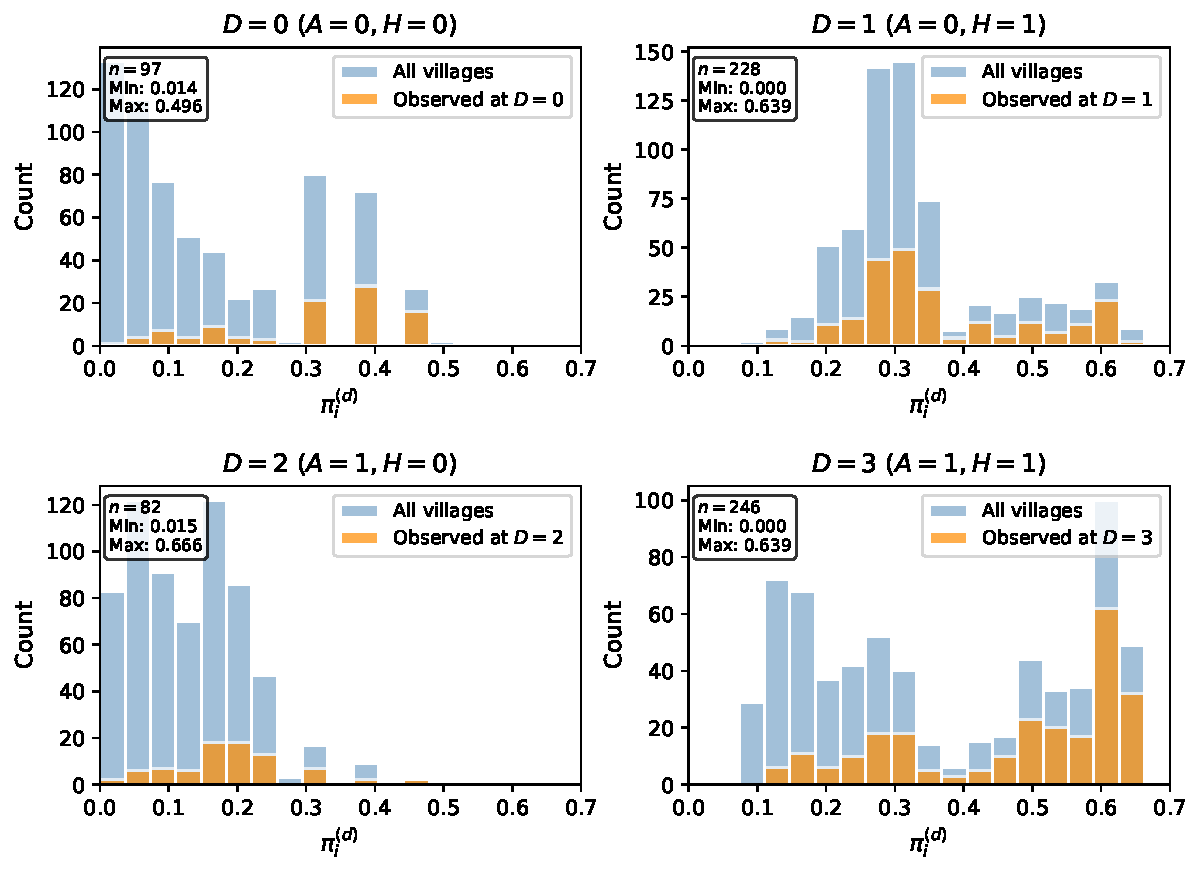
\includegraphics[width=\linewidth]{../propensity_histograms.pdf}
    \caption{Propensity score distributions by exposure level. Blue bars show the distribution of $\pi_i^{(d)}$ across all 653 villages; orange bars show the distribution among villages actually observed at exposure $D=d$.}
    \label{fig:propensity}
\end{figure}

\paragraph{95\% confidence interval widths.} Table~\ref{tab:revenue_ci_width} presents 95\% confidence interval widths for the treatment effect estimates.
\begin{table}[h!]
    \centering
    \caption{95\% confidence interval widths for the treatment effect estimates.}
    \label{tab:revenue_ci_width}
    \begin{tabular}{lcccc}
        \toprule
        Contrast & HT & H\'{a}jek & Linear & PNA-no-harm \\
        \midrule
        Direct ($H=0$) & 4762 & 3852 & 3926 & \textbf{3638} \\
        Direct ($H=1$) & 2595 & 2573 & 2521 & \textbf{2408} \\
        Spillover ($A=0$) & 3614 & 2836 & 2807 & \textbf{2677} \\
        Spillover ($A=1$) & 3743 & 3589 & 3977 & \textbf{3503} \\
        \midrule
        Average & 3679 & 3213 & 3308 & \textbf{3057} \\
        \bottomrule
    \end{tabular}
\end{table}


\paragraph{A second outcome: wage bill per enterprise.} Table~\ref{tab:wage_results} presents treatment effect estimates for wage bill per enterprise (in KES). For this outcome, the PNA-no-harm estimator requires careful initialization to achieve competitive performance. Using seed 50039 for reproducibility, PNA-no-harm achieves an average confidence interval width of 507 KES, representing a 3\% improvement over H\'{a}jek (521) and 4\% over HT (528). The estimates suggest a moderate positive direct effect when neighbors are untreated ($H=0$), with point estimates around 363 KES. All estimators find insignificant spillover effects, consistent with wage bill being less sensitive to network spillovers than revenue.

\begin{table}[h]
    \centering
    \caption{Treatment effect estimates for wage bill per enterprise (KES). * denotes statistical significance at $\alpha=0.05$. PNA results use seed 50039.}
    \label{tab:wage_results}
    \small
    \begin{tabular}{l cc cc cc cc}
        \toprule
        & \multicolumn{2}{c}{HT} & \multicolumn{2}{c}{H\'{a}jek} & \multicolumn{2}{c}{Linear} & \multicolumn{2}{c}{PNA-no-harm} \\
        \cmidrule(lr){2-3} \cmidrule(lr){4-5} \cmidrule(lr){6-7} \cmidrule(lr){8-9}
        Contrast & $\hat\tau$ & 95\% CI & $\hat\tau$ & 95\% CI & $\hat\tau$ & 95\% CI & $\hat\tau$ & 95\% CI \\
        \midrule
        Direct($H=0$) & 516* & [229, 803] & 436* & [155, 718] & 444* & [158, 730] & 363* & [94, 632] \\
        Direct($H=1$) & -95 & [-337, 146] & 11 & [-229, 250] & 28 & [-218, 274] & 16 & [-204, 237] \\
        Spillover($A=0$) & 606* & [380, 833] & 372* & [150, 594] & 321* & [81, 561] & 253* & [30, 476] \\
        Spillover($A=1$) & -5 & [-307, 297] & -54 & [-353, 245] & -29 & [-378, 321] & -66 & [-367, 235] \\
        \bottomrule
    \end{tabular}
\end{table}

\begin{table}[h]
    \centering
    \caption{95\% confidence interval widths for wage bill (KES). Boldface indicates narrowest width for each contrast.}
    \label{tab:wage_ci_width}
    \begin{tabular}{lcccc}
        \toprule
        Contrast & HT & H\'{a}jek & Linear & PNA-no-harm \\
        \midrule
        Direct($H=0$) & 574 & 563 & 572 & \textbf{538} \\
        Direct($H=1$) & 483 & 479 & 492 & \textbf{442} \\
        Spillover($A=0$) & 453 & \textbf{444} & 480 & 446 (close to best) \\
        Spillover($A=1$) & 603 & \textbf{598} & 700 & 602 (close to best)\\
        \midrule
        Average & 528 & 521 & 561 & \textbf{507} \\
        \bottomrule
    \end{tabular}
\end{table}

\end{document}

% This document was modified from the file originally made available by
% Pat Langley and Andrea Danyluk for ICML-2K. This version was created
% by Iain Murray in 2018, and modified by Alexandre Bouchard in
% 2019 and 2021 and by Csaba Szepesvari, Gang Niu and Sivan Sabato in 2022.
% Modified again in 2023 and 2024 by Sivan Sabato and Jonathan Scarlett.
% Previous contributors include Dan Roy, Lise Getoor and Tobias
% Scheffer, which was slightly modified from the 2010 version by
% Thorsten Joachims & Johannes Fuernkranz, slightly modified from the
% 2009 version by Kiri Wagstaff and Sam Roweis's 2008 version, which is
% slightly modified from Prasad Tadepalli's 2007 version which is a
% lightly changed version of the previous year's version by Andrew
% Moore, which was in turn edited from those of Kristian Kersting and
% Codrina Lauth. Alex Smola contributed to the algorithmic style files.
